\chapter{Collineations}

\section{The Collineation Group}
\begin{defn}
    A \textsl{collineation} between two affine or projective planes is a morphism of the underlying incidence geometries [cf.~Definition~\ref{defn:incidence-geometry}] whose components are both bijections.

    A collineation \textsl{of} a plane $\Pi$ is an automorphism of $\Pi$.

    A \textsl{correlation} is a a collineation from a plane to its dual.
\end{defn}

\begin{rem}
    Let $\phi$ be a collineation of the projective plane $\igeo$. Then
    \[
        \block a\in\pl(A)\iff\phi(\block a)\in\pl(\phi(A)),
    \]
    i.e., $\phi(\pl(A))=\pl(\phi(A))$, for $A\in\pts$. Dually, if $\block a\in\blocks$, then $\phi(\tr(\block a))=\tr(\phi(\block a))$.
\end{rem}

\begin{xmpl}
    Consider the projective plane $\PG(2,\kappa)$ [cf.~Example~\ref{xmpl:pg(2,k)}]. The morphism $(\phi_{\pts},\phi_{\blocks})\colon\PG(2,q)\to\PG(2,q)^*$ defined by
    \begin{align*}
        \phi_{\pts}\colon\pts&\to\blocks\\ [x_0:x_1:x_2]&\mapsto(x_0:x_1:x_2)\\
        \phi_{\blocks}\colon\blocks&\to\pts\\ (u_0:u_1:u_2)&\mapsto[u_0:u_1:u_2]
    \end{align*}
    is a correlation.
\end{xmpl}

\begin{rem}
    Since any collineation between affine planes preserves parallelism, it can be extended in a unique way to a collineation between the projective closures of the domain and the codomain.
\end{rem}

\begin{defn}
    The group of collineations of a projective plane $\Pi$ is called the \textsl{full collineation group} of $\Pi$ and denoted $\Aut(\Pi)$. The subgroups of $\Aut(\Pi)$ are called \textsl{collineation groups} of $\Pi$.
\end{defn}

\needspace{2\baselineskip}
\begin{xmpls}\label{xmpl:a-cyclic-collineation}${}$
    \begin{enumerate}[a),font=\upshape]
        \item Let $\Pi$ be the cyclic plane of $v=n^2+n+1$ points, as introduced in Example~\ref{xmpl:cyclic-planes}. The map
        \begin{align*}
            \rho\colon\Pi&\to\Pi\\
            i&\mapsto i+1\\
            R&\mapsto R+1
        \end{align*}
        is clearly a collineation of $\Pi$.

        \item The bijection of Example~\ref{xmpl:triangular-Fano} is a collineation between two representations of the Fano plane.

        \item Any nonsingular\/ $3 \times 3$ matrix\/ $A$ with entries from a field\/ $\kappa$ induces a collineation of the projective plane\/ $\PG(2,\kappa)$.

        This transformation\/ $\phi$ is defined on the points of\/ $\PG(2,\kappa)$ as
        \begin{align*}
            \phi[\vect x]=[A\vect x],
        \end{align*}
        which is well-defined because $A$ is nonsingular and respects the equivalence relation of homogeneous coordinates.
        
        The corresponding map on the lines of $\PG(2,\kappa)$ is given by
        \[
            \phi(\vect u)=(A^{-T}\vect u),
        \]
        where $A^{-T}$ denotes $(A^{-1})^T$. This means that the subspace orthogonal to~$\vect u$, i.e., the projective line defined by the orthogonal subspace generated by~$\vect u$, is mapped to the subspace orthogonal to $A^{-T}\vect u$.
        
        To see that this transformation is a collineation take a point $[x_0:x_1:x_2]$ lying on a line $(u_0:u_1:u_2)$. Then, $\vect u^T\vect x=0$ and their images, $[A\vect x]$ and $(A^{-T}\vect u)$, satisfy the same condition:
        \[
            (A^{-T}\vect u)^TA\vect x
                = \vect u^T A^{-1}A\vect x
                = \vect u^T\vect x = 0.
        \]
    \end{enumerate}
\end{xmpls}

\begin{rem}\label{rem:Fq3/Fq-projective-plane}
    As a generalization of Example c) above, if $\V$ is a $3$-dimensional vector space over $\kappa$, and the $1$- and $2$-dimensional subspaces of $\V$ define the projective plane $\PG(2,q)$, then every automorphism $\phi$ of $\V$ induces a collineation of $\PG(2,q)$. More precisely, the action of $\phi$ on the points of $\PG(2,q)$ is given by $\phi[\vect v] = [\phi(\vect v)]$, where square brackets denote projection onto the space of lines through the origin (i.e., the quotient by scalar multiples). Dually, the action of this collineation on the lines of $\PG(2,q)$ is given by $(\phi^{-1})^*$, the dual of the inverse of $\phi$. This correspondence follows directly from the equivalence between matrix transposition and duality of linear transformations.

    If $\kappa = \Fq$ and $K = \Fq[q^3]$, we can identify the projective plane $\PG(2,q)$ with the geometry of the $3$-dimensional $\kappa$-vector space $K$. Under this identification, the points of $\PG(2,q)$ correspond to the elements of $K^\times/\kappa^\times$, and every $\kappa$-linear automorphism of $K$ induces a collineation of $\PG(2,q)$.\footnote{As usual, $K^\times$ (respectively, $\kappa^\times$) denotes the multiplicative group of nonzero elements of $K$ (resp.\ $\kappa$).}
    
    For example, the expansion $\varepsilon_\alpha$, defined by $\varepsilon_\alpha(x)=\alpha x$ for $\alpha \in K^\times$, yields a collineation of $\PG(2,q)$. The action of this collineation on the lines of $\PG(2,q)$ corresponds to $(\varepsilon_\alpha^{-1})^*$.

    To see this in detail, fix $f(t)=t^3+at^2+bt+c\in\kappa[t]$ irreducible. Then, $B=(1,\tau,\tau^2)$, where $f(\tau)=0$ is a basis of $K=\kappa[t]/(f(t))$. Let $B^*=(\theta_0,\theta_1,\theta_2)$ be the dual of $B$.  If $x\in K^\times$ has coordinates $(x_0,x_1,x_2)$ in $B$, then $\varepsilon_\alpha(x)$ has coordinates $(\theta_0(\alpha x),\theta_1(\alpha x),\theta_2(\alpha x))$ in this basis. Therefore, $\varepsilon_\alpha$ maps the homogeneous coordinates $[x_0:x_1:x_2]$ to $[\theta_0(\alpha x):\theta_1(\alpha x):\theta_2(\alpha x)]$. The action of this collineation on the projective line $\block u=(u_0:u_1:u_2)$ of $\PG(2,q)$ is given by
    \begin{align*}
        (\varepsilon_{\alpha}^{-1})^*
            \colon\ker(u_0\theta_0+u_1\theta_1+u_2\theta_2)
            &\mapsto \ker((u_0\theta_0+u_1\theta_1+u_2\theta_2)
                \circ\varepsilon_{\alpha^{-1}}),
    \end{align*}
    which corresponds to the equation
    \begin{align*}
        u_0\theta_0(\alpha^{-1}x)
            + u_1\theta_1(\alpha^{-1}x)
            + u_2\theta_2(\alpha^{-1}x)=0,
    \end{align*}
    i.e.,
    \begin{align}\label{eq:action-on-lines}
        (\varepsilon_\alpha^{-1})^*(\block u)
            &= \set{[x]\mid
                [\alpha^{-1}x]\in\block u}\nonumber\\
            &= \set{[\alpha x]\mid [x]\in\block u}.
    \end{align}
    To complete the analysis, observe that
    $$
        \varepsilon_1=
            \begin{pmatrix}
                1   &0  &0\\
                0   &1  &0\\
                0   &0  &1
            \end{pmatrix}
        \quad
        \varepsilon_\tau=
            \begin{pmatrix}
                0   &0  &-c\\
                1   &0  &-b\\
                0   &1  &-a
            \end{pmatrix}
        \quad
        \varepsilon_{\tau^2}=
            \begin{pmatrix}
                0   &0  &-c\\
                1   &0  &-b\\
                0   &1  &-a
            \end{pmatrix}^{\!\!\!2}
    $$
    where
    $$
        \begin{pmatrix}
            0   &0  &-c\\
            1   &0  &-b\\
            0   &1  &-a
        \end{pmatrix}^{\!\!\!2}
        =
        \begin{pmatrix}
             0 & -c & ac\\
             0 & -b & ab-c\\
             1 & -a & a^2-b 
        \end{pmatrix}.
    $$
    Hence, if $\alpha=c_0+c_1\tau+c_2\tau^2$, we have
    $$
        \varepsilon_\alpha=c_0\varepsilon_1+c_1\varepsilon_\tau
            +c_2\varepsilon_{\tau^2}
            = \begin{pmatrix}
                    c_0 & -c_2c & c(c_2a - c_1) \\
                    c_1 & c_0 - c_2b & -c_1b + c_2(ab-c) \\
                    c_2 & c_1 - c_2a & c_0 - c_1a + c_2(a^2-b)
                \end{pmatrix}
    $$
    
    \small
    For instance, in $\Fq[7]$ we can take $f(t)=t^3-2$. Thus, $a=b=0$ and $c=-2$, which yield
    \begin{align*}
        \varepsilon_\alpha=\begin{pmatrix}
            c_0     &2c_2      &2c_1\\
            c_1     &c_0    &2c_2\\
            c_2     &c_1    &c_0
        \end{pmatrix}.\\
    \end{align*}
    Similarly, in the case where $\kappa=\Fq[2^2]$, we can take $f(t)=t^3+i$ and obtain $a=b=0$ and $c=i$. Thus,
    \[
        \varepsilon_\alpha=\begin{pmatrix}
            c_0     &ic_2       &ic_1\\
            c_1     &c_0        &ic_2\\
            c_2     &c_1        &c_0
        \end{pmatrix}.
    \]

    \normalsize
\end{rem}


\section{Fixed Elements of Collineations}

\begin{defns}
    Let $\phi$ be a collineation of the plane $\Pi$. A point $P$ is a \textsl{fixed point} of $\phi$ if $\phi(P)=P$. Similarly, a line $\block a$ is \textsl{fixed by} $\phi$ if $\phi(\block a)=\block a$.

    In what follows, $\Fix\phi$ will denote the set of all points and lines fixed by~$\phi$.

    A set $\mathbf C$ consisting of points and lines of a projective plane is called a \textsl{closed configuration} if it satisfies
    \begin{enumerate}[label=C\arabic*.]
        \item $A,B\in\mathbf C\implies AB\in\mathbf C$
        \item $\block a,\block b\in\mathbf C\implies \block a\wedge\block b\in\mathbf C$.
    \end{enumerate}
\end{defns}

\begin{rem}
    If\/ $\phi$ is a collineation of a projective plane, then\/ $\Fix\phi$ is a closed configuration.
\end{rem}

\begin{prop}\label{prop:Fix-subplane-4-points-condition}
    Let\/ $\phi$ be a collineation of a projective plane\/ $\Pi$. Then\/ $\Fix\phi$ is a subplane of\/ $\Pi$ if, and only if, it contains four points in general position.
\end{prop}

\begin{proof}
    By the previous remark, $\Fix\phi$ satisfies axioms \ref{P1} and \ref{P2}. Therefore, the conclusion is a direct consequence of Lemma~\ref{lem:alternative-projective-axiom}.
\end{proof}

\begin{rem}
    If\/ $\Fix\phi$ is a subplane of\/ $\Pi$, then the number of fixed points equals the number of fixed lines. As we shall see, this equality holds even when\/ $\Fix\phi$ is not a subplane.
\end{rem}

\begin{rem}
    Note that the inclusion of a proper subplane into a plane is not a collineation, as collineations are bijective by definition.
\end{rem}

\begin{defn}
    A \textsl{permutation matrix} is a square binary matrix that has precisely one entry equal to $1$ in each row and each column.
\end{defn}

\begin{rem}
    Permutation matrices correspond to linear automorphisms of~$\kappa^n$ which permute coordinates. More precisely, if $\sigma\in S_n$, the matrix $P_\sigma$ of the automorphism $(x_1,\dots,x_n)\mapsto(x_{\sigma(1)},\dots,x_{\sigma(n)})$ in the canonical basis, is the permutation matrix associated to $\sigma$. Note also that $\det P_{\sigma}=\sg(\sigma)$. In particular,
    \begin{align*}
        C_j(P_\sigma) &= P_\sigma\vect e_j\\
            &= (\delta_{j\sigma(1)},\dots,\delta_{j\sigma(n)})\\
            &= \vect e_{\sigma^{-1}(j)}\\
            &= C_{\sigma^{-1}(j)}(\op{Id}),
    \end{align*}
    where $C_j$ is the map that extracts the $j$th column of a matrix, and $\vect e_j$ is the $j$th canonical vector $(\delta_{j1},\dots,\delta_{jn})$.

    Since any permutation of the canonical basis is an orthonormal basis, the matrix $P_\sigma$ is orthonormal, i.e., $P_\sigma^T=P_\sigma^{-1}$.

    Since
    \begin{align*}
        P_\sigma P_\omega\vect e_j
            &= P_\sigma\vect e_{\omega^{-1}(j)}\\
            &= \vect e_{\sigma^{-1}\omega^{-1}(j)}\\
            &= \vect e_{(\omega\sigma)^{-1}(j)}\\
            &= P_{\omega\sigma}\vect e_j,
    \end{align*}
    and $P_{\id}=\id$, we obtain
    $$
        P_{\sigma^{-1}}=P_\sigma^{-1}=P_\sigma^T.
    $$
\end{rem}

\begin{test}
    If $\sigma$ is the cycle $(132)$, then $\sigma^{-1}=(123)$ and so
    $$
        P_\sigma=\begin{bmatrix}
                0   &0  &1\\
                1   &0  &0\\
                0   &1  &0
            \end{bmatrix}.
    $$
    Conversely,
    $$
        \begin{bmatrix}
                x_{\sigma(1)}\\
                x_{\sigma(2)}\\
                x_{\sigma(3)}
            \end{bmatrix}
            = \begin{bmatrix}
                x_3\\
                x_1\\
                x_2
            \end{bmatrix}
            = \begin{bmatrix}
                0   &0  &1\\
                1   &0  &0\\
                0   &1  &0
            \end{bmatrix}\begin{bmatrix}
                x_1\\
                x_2\\
                x_3
            \end{bmatrix}\!\!.
    $$
    Moreover,
    $$
        \begin{bmatrix}
                x_{\sigma^{-1}(1)}\\
                x_{\sigma^{-1}(2)}\\
                x_{\sigma^{-1}(3)}
            \end{bmatrix}
            = \begin{bmatrix}
                x_2\\
                x_3\\
                x_1
            \end{bmatrix}
            = \begin{bmatrix}
                0   &0  &1\\
                1   &0  &0\\
                0   &1  &0
            \end{bmatrix}\begin{bmatrix}
                x_1\\
                x_2\\
                x_3
            \end{bmatrix}\!\!.
    $$
\end{test}

\begin{rem}
    Let  $\Pi=\igeo$ be a finite projective plane of order $n$. Put $v=n^2+n+1$ and $\pts=\set{P_1,\dots,P_v}$. If $\phi$ is a collineation of $\Pi$, then the $v\times v$ matrix $P=(p_{ij})_{1\le i,j\le n}$, where
    $$
        p_{ij}=\begin{cases}
            1   &\text{if }\phi(P_i)=P_j,\\
            0   &\text{otherwise}
        \end{cases}
    $$
    is a permutation matrix. In fact, it is the permutation matrix associated with the permutation that $\phi$ defines on $\pts$.

    Dually, we obtain the permutation matrix $Q$ with entries
    $$
        q_{ij}=\begin{cases}
            1   &\text{if }\phi(\block a_i)=\block a_j,\\
            0   &\text{otherwise}
        \end{cases}
    $$
    where $\blocks=\set{\block a_1,\dots,\block a_v}$.

    The matrices $P$ and $Q$ are said to be \textsl{induced} by $\phi$.
\end{rem}

\begin{thm}
    Let\/ $\Pi=\igeo$ be a finite projective plane with incidence matrix\/ $A$. Then a pair of permutations\/ $\phi_1\in\Sym(\pts)$ and\/ $\phi_2\in\Sym(\blocks)$ defines a collineation of\/ $\Pi$ if, and only if, their permutation matrices\/ $P$ and\/ $Q$ satisfy\/ $AP = QA$.
\end{thm}

\begin{proof}
    With the notation of the previous remark, $A=(a_{ij})_{1\le i,j\le v}$ where
    $$
        a_{ij}\ne0\iff a_{ij} = 1 \iff P_j\incidence\block a_i
            %\iff \phi(P_j)\incidence\phi(\block a_i).
    $$
    We have,
    $$
        (AP)_{ij} = \sum_{k=1}^va_{ik}p_{kj}=a_{ij'}
        \text{ for } \phi_1(P_{j'})=P_j.
    $$
    Therefore,
    $$
        (AP)_{ij}\ne0\iff(AP)_{ij}=1
            \iff P_{j'}\incidence\block a_i,\;\phi_1(P_{j'})=Pj
            \iff \phi_1^{-1}(P_j)\incidence\block a_i.
    $$
    On the other hand,
    $$
        (QA)_{ij} = \sum_{k=1}^vq_{ik}a_{kj}=a_{i'j}
        \text{ for } \phi_2(\block a_i)=\block a_{i'}.
    $$
    Hence,
    $$
        (QA)_{ij}\ne0\iff(QA)_{ij}=1
            \iff P_j\incidence \phi_2(\block a_i).
    $$
    Then, $AP=QA$ if, and only if, for all $0\le i,j\le v$ we have
    $$
        \phi_1^{-1}(P_j)\incidence\block a_i
            \iff P_j\incidence \phi_2(\block a_i),
    $$
    which means that $(\phi_1,\phi_2)$ is a collineation.
    %
    
\end{proof}

\begin{cor}\label{cor:fixed-points-equals-fixed-lines}
    Let\/ $\phi$ be a collineation of a finite projective plane. Then the number of fixed points of\/ $\phi$ equals the number of fixed lines.
\end{cor}

\begin{proof}
    Using the same notation as above, $P_j$ is fixed if, and only if, $p_{jj}=1$. Similarly $\block a_i$ is fixed if, and only if, $q_{ii}=1$. Thus, the number of fixed points coincides with $\tr(P)$ and the number of fixed lines with $\tr(Q)$. Since $QA=AP$ and $A$ is nonsingular [cf.~Lemma~\ref{lem:characteristic-polynomial-AA^T-projective-plane}], $Q=APA^{-1}$, which shows that $P$ and $Q$ have the same trace.
    %
    
\end{proof}

\begin{ntn}
    Let\/ $X$ be a finite set. The set of bijections of\/ $X$ is denoted by\/ $\Sym(X)$.
    
    If\/ $G$ is a subgroup of\/ $\Sym(X)$, given\/ $x\in X$, its \textsl{orbit} is\/ $\mathcal O_x=\set{g(x)\mid g\in G}$, and\/ $G_x=\set{g\in G\mid g(x)=x}$ its \textsl{stabilizer}.

    The group\/ $G$ is \textsl{transitive} if\/ $\mathcal O_x=X$ for some, and a fortiori every, $x\in X$.

    The group\/ $G$ is \textsl{regular} if it is transitive and\/ $G_x=\set\id$ for every\/ $x\in X$.
\end{ntn}

\begin{lem}\label{lem:fundamental-counting-principle}
    Let\/ $X$ be a finite set and\/ $G$ a subgroup of\/ $\Sym(X)$. Then, $|\mathcal O_x||G_x|=|G|$, for every\/ $x\in X$.
\end{lem}

\begin{proof}\citep[Fundamental Counting Principle]{LC-Groups}
    Fix $x\in X$. Consider the equivalence relation in $G$ defined by
    $$
        g\sim h\iff g(x)=h(x).
    $$
    Since,
    $$
        g\sim h\iff h^{-1}g\in G_x,
    $$
    we deduce that the class of $g$ in $G/{\sim}$ has $|G_x|$ elements. Since the map $G\to\mathcal O_x$, given by $g\mapsto g(x)$, induces a bijection $G/{\sim}\to\mathcal O_x$, the conclusion is clear.
    %
\end{proof}

\begin{thm}\label{thm:number-of-orbits}
    Let\/ $X$ be a finite set and $G$ a subgroup of\/ $\Sym(X)$. For each\/ $g\in G$ let\/ $\chi(g)$ denote the number of elements of\/ $X$ fixed by\/ $g$, and let\/~$t$ be the number of orbits of\/ $G$ on\/ $X$. Then
    \[
        t|G| = \sum_{g\in G}\chi(g).
    \]
\end{thm}

\begin{proof}
    Consider the set
    $$
        F = \set{(x,g)\in X\times G\mid g(x)=x}.
    $$
    Given $x\in X$, let $G_x=\set{g\in G\mid g(x)=x}$ be its \textsl{stabilizer}. Then,
    $$
        F = \bigcup_{x\in X}\set x\times G_x
    $$
    is a partition of $F$. Therefore,
    $$
        |F|=\sum_{x\in X}|G_x|.
    $$
    There is another partition
    $$
        F = \bigcup_{g\in G}X_g\times\set g,
    $$
    where $X_g=\set{x\in X\mid g(x)=x}$. Hence,
    $$
        \sum_{g\in G}\chi(g)=\sum_{x\in X}|G_x|.
    $$
    By the lemma, $|G_x||\mathcal O_x|=|G|$. Thus,
    \[
        \sum_{g\in G}\chi(g)
            =|G|\sum_{x\in X}\frac1{|\mathcal O_x|}.
            \tag{$\ast$}
    \]
    Since $y\in\mathcal O_x\comm \mathcal O_y=\mathcal O_x$, a representation $\set{\mathcal O_{x_1},\dots,\mathcal O_{x_t}}$ of the orbits of $X$ is a partition of $X$. Thus,
    $$
        \sum_{x\in X}\frac1{|\mathcal O_x|}
            = \sum_{i=1}^t\sum_{x\in\mathcal O_{x_i}}
                \frac1{|\mathcal O_{x_i}|}
            = \sum_{i=1}^t|
                \mathcal O_{x_i}|\frac1{|\mathcal O_{x_i}|}
            = t.
    $$
    The conclusion is now an immediate consequence of $(\ast)$.
    %
\end{proof}

\begin{cor}\label{cor:point-and-line-orbits}
    Let\/ $G$ be a collineation group of a finite projective plane. Then the number of point orbits and the number line orbits are equal.
\end{cor}

\begin{proof}
    Let\/ $\Pi=\igeo$ be the projective plane under consideration, and let\/ $t_{\pts}$ and\/ $t_{\blocks}$ denote the number of point and line orbits, respectively. For each\/ $\phi\in G$, let\/ $\chi_{\pts}(\phi)$ and\/ $\chi_{\blocks}(\phi)$ be the number of points and lines fixed by\/ $\phi$. Since\/ $G$ acts as a subgroup of both\/ $\Sym(\pts)$ and\/ $\Sym(\blocks)$, the theorem yields
    \[
        t_{\pts}|G| = \sum_{\phi\in G} \chi_{\pts}(\phi)
        \quad\text{and}\quad
        t_{\blocks}|G| = \sum_{\phi\in G} \chi_{\blocks}(\phi).
    \]
    The conclusion now follows directly from Corollary~\ref{cor:fixed-points-equals-fixed-lines}.
\end{proof}

\begin{cor}\label{cor:point-line-transitivity}
    A group of collineations of a finite projective plane is transitive on the points if, and only if, it is transitive on the lines of the plane.
\end{cor}

\begin{proof}
    This is a direct consequence of Corollary~\ref{cor:point-and-line-orbits}.
\end{proof}

\section{Singer Groups and Cyclic Planes}

\begin{defn}
    Let\/ $G$ be a finite group of order\/ $v$, written additively. A subset\/ $D\subseteq G$ with\/ $k$ elements is called a\/ \textsl{$(v,k,\lambda)$-difference set} if every nonzero element of\/ $G$ can be expressed as a difference\/ $d_1 - d_2$ of two distinct elements in\/~$D$ in exactly\/~$\lambda$ ways. A difference set is called \textsl{perfect} when\/ $\lambda = 1$.
\end{defn}

%\needspace{2\baselineskip}
\begin{xmpls}\label{xmpls:difference-sets}${}$
    \begin{enumerate}[a)]
        \item {[Fano's difference set]} Consider the Fano plane [cf.~Example~\ref{xmpl:Fano}], the projective plane of order $2$, which also can be visualized as
        $$
            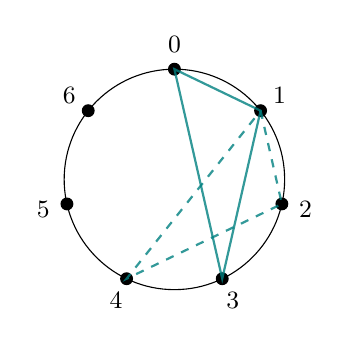
\begin{tikzpicture}[
                scale=0.7,
                point/.style={circle, fill=black, inner sep=1.5pt, draw=black},
                line_style/.style={thick, opacity=0.8, color=teal}
            ]
            \def\r{2};
            \draw (0,0) circle (\r);
            
            % --- Define the 7 points on a circle ---
            \foreach \i in {0,...,6} {
                % Calculate angle in degrees (starting from top and going clockwise)
                \pgfmathsetmacro{\angle}{90 - \i * 360 / 7}
                
                % Calculate coordinates on the circle
                \pgfmathsetmacro{\x}{\r*cos(\angle)}
                \pgfmathsetmacro{\y}{\r*sin(\angle)}
                
                % Define the point
                \coordinate (p\i) at (\x, \y);
                % Place point
                \node[point] at (p\i) {};
                
                % Calculate label position slightly outside the circle
                \pgfmathsetmacro{\labelx}{1.22 * \x}
                \pgfmathsetmacro{\labely}{1.22 * \y}
                % Place label
                \node at (\labelx, \labely) {\small$\i$};
            }
        
            % --- Draw a couple of lines (the translates of the difference set {0,1,3}) ---
            % Each line is a triangle connecting three points.
            \draw[line_style] (p0) -- (p1) -- (p3) -- cycle;
            \draw[line_style, dashed] (p1) -- (p2) -- (p4) -- cycle;
            \end{tikzpicture}
        $$
        Consider the collineation group
        $$
            D = \set{\rho^r\mid r=0,1,3}
        $$
        where $\rho$ is the collineation defined in Example~\ref{xmpl:a-cyclic-collineation}, i.e., the collineation that satisfies $\rho(i)=i+1$. Since the cyclic group generated by $\rho$ is isomorphic to the additive group $\Z_7$, to verify that $D$ is a perfect difference set, it is enough to show that the set of exponents $\set{0,1,3}$ defines a $(7,3,1)$-difference set in the additive group $\Z_7$, as verified here
        \[
            \begin{array}{c|ccccc}
                - &0 &1 &3\\
                \hline\rule{0pt}{11pt}
                0 &0 &6 &4\\
                1 &1 &0 &5\\
                3 &3 &2 &0
            \end{array}
        \]

        \item {[Paley's Difference Set of Order 11]} In the additive group of residues modulo $11$ consider the set of nonzero squares
        $$
            D = \set{m^2\mid m\in \Z_{11}\setminus\set0}
                = \set{1,3,4,5,9}.
        $$
        This is a $(11,5,2)$-difference set:
        \[
            \begin{array}{c|ccccc}
                - &1 &3 &4 &5 &9 \\
                \hline\rule{0pt}{11pt}
                1 &0 &9 &8 &7 &3 \\
                3 &2 &0 &10  &9 &5 \\
                4 &3 &1 &0 &10 &6 \\
                5 &4 &2 &1 &0 &7 \\
                9 &8 &6 &5 &4 &0
            \end{array}
        \]
        This difference set is the basis of the $2$-$(11,5,2)$ design $\igeo$ where
        $$
            \pts=\Z_{11},
            \quad
            \blocks=\set{D+i\mid i\in\Z_{11}},
        $$
        and $\incidence$ is the membership relation. Given two points $m\ne m'$, we have
        $$
            m=d+i,\; m'=d'+i
                \iff m-m'=d-d',\; i=m-d=m'-d',
        $$
        which admits two solutions for $d$ and $d'$ in $D$, say $(d_1,d'_1)$ and $(d_2,d'_2)$. Therefore, $i_1=m-d_1=m'-d_1'$ and $i_2=m-d_2=m'-d'_2$ induce the translations of $D$ that define the two blocks incident with $m$ and $m'$.
        
        For instance, in the case $m=2$ and $m'=7$, we have
        \begin{align*}
            m-m'=\begin{cases}
                9-3\\4-9
            \end{cases}
                \implies\begin{cases}
                    i_1=2-9=7-3=4,\\
                    i_2=2-4=7-9=9,
                \end{cases}
        \end{align*}
        yielding $\set{m,m'}=D+4\cap D+9$.
    \end{enumerate}
\end{xmpls}

\begin{defn}
    A \textsl{Singer group} of a projective plane is a collineation group that is cyclic and acts regularly on its points. A plane that has a Singer group is called a \textsl{cyclic} plane. The generators of a Singer group are called \textsl{Singer cycles}.
\end{defn}

\begin{rem}
    In other words, a Singer group is a cyclic group of collineations such that, given a generator $\xi$ and any pair of points $(A,B)$, there exists a unique integer $0 \le j < \ord(\xi)$ satisfying $B = \xi^j(A)$.
    
    Note also that the order of a Singer group is $v=q^2+q+1$, where $q$ is the order of the projective plane.
\end{rem}

\begin{xmpl}
    The cyclic group generated by the collineation $\rho$ of Examples~\ref{xmpl:a-cyclic-collineation} and~\ref{xmpls:difference-sets} acts regularly on the points of the Fano plane. First, it acts transitively on the points because $\rho^{j-i}(i)=i+j-i=j$. Second, if $\rho^r(i)=i$, then $i+r=i$, which implies $r=0$ and $\rho^r=\id$. In consequence, the cyclic group generated by $\rho$ is a Singer group and the Fano plane is a cyclic plane.
\end{xmpl}

\begin{thm}
    The plane\/ $\PG(2,q)$ possesses a cyclic Singer group isomorphic to the additive group\/ $\Z_v$, with $v=q^2+q+1$. The set of points on any line of the plane corresponds to a planar difference set in the group\/ $\Z_v$.
\end{thm}

\begin{proof}
    Let $\kappa=\Fq$ and put $K=\mathbb{F}_{q^3}$. According to Remark~\ref{rem:Fq3/Fq-projective-plane}, $\PG(2,q)$ can be identified with the $\kappa$-vector space $K$. Under this identification, the points of $\PG(2,q)$ correspond to the elements of $K^\times/\kappa^\times$.

    For each $\alpha \in K^\times$, the expansion $\varepsilon_\alpha$ yields a collineation of $\PG(2,q)$. This defines a group homomorphism:
    \begin{align*}
        \varepsilon\colon K^\times&\to\Aut(\PG(2,q))\\
        \alpha&\mapsto\varepsilon_\alpha.
    \end{align*}
    Let $G=\im(\varepsilon)$. Then $G$ is a collineation group of $\PG(2,q)$. The action of $\varepsilon_\alpha$ on the points of $\PG(2,q)$ is given by $\varepsilon_\alpha([x])=[\alpha x]$, where square brackets indicate projection modulo $\kappa^\times$.
    
    We claim that $G$ acts regularly on the points of $\PG(2,q)$.
    
    First, consider the stabilizer of a point $[x] \in \PG(2,q)$ in the group $G$. An element $\varepsilon_\alpha \in G$ fixes $[x]$ if $\varepsilon_\alpha([x])=[x]$, which means $[\alpha x]=[x]$. This implies that $\alpha x = \lambda x$ for some $\lambda \in \kappa^\times$. Since $x \ne 0$, it follows that $\alpha = \lambda$, and thus $\varepsilon_\alpha$ is the identity collineation. Therefore, the stabilizer $G_{[x]}$ consists only of the identity element of $G$.
    
    Second, we show that $G$ acts transitively on the points of $\PG(2,q)$. Let $[x]$ and $[y]$ be any two points in $\PG(2,q)$. We need to find an $\alpha \in K^\times$ such that $\varepsilon_\alpha([x])=[y]$, i.e., $[\alpha x]=[y]$. This means $\alpha x = \lambda y$ for some $\lambda \in \kappa^\times$. Since $x,y \in K^\times$, we can choose $\alpha = y x^{-1}$. Thus, $G$ acts transitively.
    
    Since $G$ acts transitively and has a trivial stabilizer for each point, $G$ is a regular collineation group on the points of $\PG(2,q)$.
    
    Finally, since $K^\times$ is cyclic (as the multiplicative group of a finite field), and~$\varepsilon$ induces by coastriction an epimorphism from $K^\times$ to $G$, the collineation group $G$ must also be cyclic. As $G$ is a cyclic collineation group that acts regularly on the points of $\PG(2,q)$, it is a Singer group.

    Clearly, $\ker\varepsilon=\kappa^\times$. Hence, $G\cong K^\times/\kappa^\times$, and so $|G|=(q^3-1)/(q-1)=v$. Therefore, $G$, being cyclic, is isomorphic to~$\Z_v$. More precisely, if $\sigma$ is a primitive element of $K^\times$, then $\varepsilon_\sigma$ is a Singer cycle and, given a point $A_0\in\PG(2,q)$, every other point has the form $A_i=\varepsilon_{\sigma^i}(A_0)$ for $0\le i<v$.

    By Corollary~\ref{cor:point-line-transitivity}, $G$ acts transitively on the lines of $\PG(2,q)$. Hence, if $\block u$ is a line, its orbit $\mathcal{O}_{\block u}$ under the action of $G$ coincides with the entire set of lines. It follows from Lemma~\ref{lem:fundamental-counting-principle} that
    \[
        |G_{\block u}| = \frac{|G|}{|\mathcal{O}_{\block u}|} = 1,
    \]
    which shows that $G$ acts regularly on the lines of $\PG(2,q)$.

    It remains to be seen that the set of points on any line corresponds to a planar difference set in the group\/ $\Z_v$.

    Fix an arbitrary point $A_0$ and label the points of the plane by $A_m = \sigma^m(A_0)$ for $m \in \Z_v$, where $v = q^2+q+1$.

    Let $\block{u}$ be any line in the plane. We define the set $D$ as the set of indices corresponding to the points on $\block{u}$:
    \[
        D = \{i \in \Z_v \mid A_i \in \block{u}\}.
    \]
    We will show that $D$ is a $(v, q+1, 1)$-difference set in the additive group $\Z_v$.
    
    First, the size of the set is $|D|=q+1$ because $\block u$ contains exactly $q+1$ points.
    
    Second, we must show that $D$ is totally irregular\footnote{Meaning that every nonzero difference in $\Z_v$ is represented by at most one pair of elements from D [cf.~Example~\ref{xmpl:cyclic-planes}].}. Suppose otherwise. Then some positive difference $d$ between elements of $D$ occurs more than once. That is, there exist two distinct pairs $(i,j)$ and $(i',j')$ of elements of $D$ such that
    \[
        j - i \equiv d \pmod{v}
        \quad\text{and}\quad
        j' - i' \equiv d \pmod{v}.
    \]
    By our labeling of the points, this implies that $A_j = \varepsilon_{\sigma^d}(A_i)$ and $A_{j'} = \varepsilon_{\sigma^d}(A_{i'})$. Since $(i,j)\ne(i',j')$, we must have $i \ne i'$ and $j \ne j'$. Hence, $\block u = A_iA_{i'} = A_jA_{j'}$, and it follows that $\varepsilon_{\sigma^d}(\block u) = \block u$. Therefore, $\varepsilon_{\sigma^d} \in G_{\block u} = \set\id$, implying $d = 0$, a contradiction.


    Thus, every nonzero difference in $\Z_v$ is represented by at most one pair of elements from $D$. Since there are $(q+1)q$ such ordered pairs and, at most, $v-1$ nonzero differences to be formed, the equality $v=q^2+q+1$ implies that each difference must be represented exactly once. Therefore, $D$ is a $(v,q+1,1)$-perfect difference set.
    
\end{proof}

\section{Central Collineations}

\begin{defn}
    Let\/ $\phi$ be a collineation of a projective plane. A point\/ $C$ is a \textsl{center} of\/ $\phi$ if each line through\/ $C$ is a fixed line of\/ $\phi$. A line\/ $\block a$ is an \textsl{axis} of\/ $\phi$ if each point on\/ $\block a$ is a fixed point of\/ $\phi$. Center and axis are dual notions.
\end{defn}


\begin{lem}\label{lem:unique-axis-center}
    If a collineation has two distinct axes, it is the identity.
\end{lem}

\begin{proof}
    Consider a collineation $\phi$ with two axes $\block a\ne\block b$.
    $$
        \begin{tikzpicture}[
            scale=0.8,
            point/.style={circle, fill=black, inner sep=1.5pt, draw=black},
            fixed_point/.style={point, fill=blue!70!black},
            axis_line/.style={thick, draw=blue!60!black},
            other_line/.style={thick, green!30!black},
            label_style/.style={font=\small,black},
            fixed_label/.style={font=\small, text=blue!70!black},
            ]
        
            \coordinate (a_start) at (-0.5,0.5);
            \coordinate (a_end) at (7.0,1.0);
            \coordinate (b_start) at (0.5,0.1);
            \coordinate (b_end) at (6.5,4.5);
            
            \path[name path=a] (a_start) -- (a_end);
            \draw[axis_line] (a_start) -- (a_end)
                node[above right, label_style] {$\block a$}
                node[pos=0.5, point, label=below right:$A$] (A) {}
                node[pos=0.85, point, label=below:$A'$] (A') {};
            
            \path[name path=b] (b_start) -- (b_end);
            \draw[axis_line] (b_start) -- (b_end)
                node[below right, label_style] {$\block b$}
                node[pos=0.80, point, label=left:$B$] (B) {}
                node[pos=0.5, point, label=above:$B'$] (B') {};
            
            \draw[other_line,name path=c] ($(A)!-0.3!(B)$) -- ($(A)!1.2!(B)$) node[label_style,left] {$\block c$};
            \draw[other_line,name path=c'] ($(A')!-0.3!(B')$) -- ($(A')!1.3!(B')$) node[label_style,above left] {$\block c'$};
            
            \path[name intersections={of=a and b, by= P}];
              
            \node[fixed_point, label={below right:$P$}] at (P) {};
            
            \path[name intersections={of=c and c', by=Q}];
            \node[point, label={right:$Q$}] at (Q) {};
        \end{tikzpicture}
    $$
    Let $P=\block a\wedge\block b$. Then $\phi(P)=P$. Let $Q$ be any point not in $\block a\cup\block b$. By axiom~\ref{P4}, we can take two lines, $\block c$ and $\block c'$, passing through $Q$ not incident with $P$. Then $A=\block a\wedge\block c$, $A'=\block a\wedge\block c'$, $B=\block b\wedge\block c$ and $B'=\block b\wedge\block c'$ belong to $\Fix\phi$, and are in general position. The result is now a direct consequence of Proposition~\ref{prop:Fix-subplane-4-points-condition}.
    %
    
\end{proof}

\begin{lem}\label{lem:fixed-not-axis-is-center}
    Let\/ $\phi$ be a collineation of a projective plane. If the line\/ $\block a$ is an axis of\/ $\phi$ and\/ $F$ is a fixed point of\/ $\phi$ not incident with\/ $\block a$, then\/ $F$ is a center of\/~$\phi$.
\end{lem}

\begin{proof}
    Let $\block b$ be a line passing through $F$. Then $A=\block a\wedge\block b$ is well-defined and belongs to $\Fix\phi$. Since $\block b=AF$, we deduce that $\block b$ is in $\Fix\phi$ too.
\end{proof}

\begin{lem}\label{lem:P-and-phi(P)}
    Let\/ $\phi$ be a collineation of a projective plane.
    \begin{enumerate}[a),font=\upshape]
        \item Suppose that\/ $C$ is a center of\/ $\phi$. Then for any point\/ $P \ne C$, the line\/ $CP$ contains the point\/ $\phi(P)$.
        \item Suppose that\/ $\block a$ is an axis of\/ $\phi$. If\/ $P\notin\Fix\phi$, then the line\/ $P\phi(P)$ is in\/ $\Fix\phi$.
    \end{enumerate}
\end{lem}

\begin{proof}${}$
    \begin{enumerate}[a)]
        \item If $P\ne C$, then $\phi(P)\in\phi(CP)=CP$ because $CP\in\Fix\phi$.

        \item Let $\block b=P\phi(P)$. Then $\block b\ne\block a$ because $P\notin\Fix\phi$. Let $B=\block b\wedge\block a$. Then, $B\in\Fix\phi$ and $\block b=PB$. Since $B\ne\phi(P)$ because $B\ne P$, we have $\phi(\block b)=\phi(P)B=\block b$ since $B\in\block b$. \qedhere
    \end{enumerate}
\end{proof}

\begin{thm}\label{thm:axis-iff-center}
    Let\/ $\phi$ be a collineation of a projective plane. If\/ $\phi$ has an axis, then it has a center.
\end{thm}

\begin{proof}
    Suppose\/ $\phi$ has an axis $\block a$. If\/ $\phi$ fixes a point $F$ not incident with $\block a$, then $F$ is a center by Lemma~\ref{lem:fixed-not-axis-is-center}.

    Assume instead that all fixed points lie in $\block a$. Let $P$ and $Q$ be two distinct points not on $\block a$. For clarity, write $X'$ for the image of a point $X$ under $\phi$.

    We claim that $C=PP'\wedge QQ'$ is a center of\/ $\phi$. Since\/ $PP'$ and\/ $QQ'$ are fixed lines by Lemma~\ref{lem:P-and-phi(P)}, it follows that\/ $C\in\Fix\phi$ and hence\/ $C\in\block a$. Let $\block b$ be any other line through $C$, and pick a point $R\ne C$ on $\block b$. Again, Lemma~\ref{lem:P-and-phi(P)} implies that\/ $RR'$ is fixed. Thus, the point\/ $D=PP'\wedge RR'$ lies on\/ $\block a$ and on\/ $PP'$, so\/ $D=C$.

    Since\/ $D\in RR'$, the \rr gives\/ $R'\in DR=CR$, hence
    \[
        \phi(\block b)=\phi(CR)=CR'=CR=\block b.
    \]
    This shows that every line through $C$ is fixed by\/ $\phi$, and so $C$ is a center.
    %
    
\end{proof}

\begin{defn}
    A collineation\/ $\alpha$ is \textsl{central-axial} if it has both a center and an axis. If\/ $C$ is a center and\/ $\block a$ is an axis of\/ $\alpha$, then\/ $\alpha$ is also called a \textsl{$(C, \block a)$-perspectivity}.

    A \textsl{$(C, \block a)$-perspectivity} is an \textsl{elation} if\/ $C \incidence \block a$, otherwise it is called a \textsl{homology}. The identity can be considered as both an elation and a homology.
\end{defn}

\begin{xmpls}${}$
    \begin{enumerate}[a)]
        \item Consider the matrix
        \[
            A = \begin{pmatrix}
                1   &2  &0\\
                0   &1  &0\\
                0   &0  &1
            \end{pmatrix}.
        \]
        Since it is nonsingular, it defines a collineation $\alpha$ in $\PG(2,\kappa)$, as shown in Example~\ref{xmpl:a-cyclic-collineation}~c). Since the transposed inverse of $A$ is
        \[
            (A^{-1})^T = \begin{pmatrix}
                \phantom-1 & 0 & 0 \\
                -2 & 1 & 0 \\
                \phantom-0 & 0 & 1
            \end{pmatrix},
        \]
        in homogeneous coordinates, $\alpha$ is given by
        \[
            \alpha[x:y:z]=[x+2y:y:z]
            \quad\text{and}\quad
            \alpha(u:v:w)= (u:-2u+v:w).
        \]
        Since (the set of eigenvalues) $\spec(A)=\set1$, the unique eigenspace of $A$ is given by the kernel of $A-I$, i.e., by the equation $2y=0$. If $2\ne0$ in $\kappa$, this is the same as $y=0$, which corresponds to the line $(0:1:0)$. In other words, $(0:1:0)$ is an axis of $\alpha$ (all the points in this line are fixed).
    
        Similarly, the eigenspace of $(A^{-1})^T$ for its eigenvalue $1$ is given by $-2u=0$ or $u=0$ if $2\ne0$. Thus, the lines $(0:v:w)$ are fixed and they all intersect at $[1:0:0]$, which is the center of~$\alpha$.
    
        Since $[1:0:0]\incidence(0:1:0)$, we see that $\alpha$ is an elation.

        \item Suppose, as before, that $2\ne0$ in $\kappa$ and let $\beta$ be the collineation of $\PG(2,\kappa)$ defined by the matrix
        \[
            B = \begin{pmatrix}
                2   &0  &0\\
                0   &2  &0\\
                0   &0   &1
            \end{pmatrix}.
        \]
        Then $\spec(B)=\set{1,2}$, where the eigenspace associated to the eigenvalue~$1$ corresponds to the fixed point $[0:0:1]$, which is the center. The other eigenspace has dimension $2$ and corresponds to the axis. However, this can be deduced from the component of $\beta$ that acts on lines and is associated to the matrix $(B^{-1})^T$. Here the $\spec$ is $\set{1,2^{-1}}$. The eigenspace of eigenvalue~$1$ is $(0:0:1)$, which corresponds to the axis. The other eigenspace has dimension $2$ and refers to all lines passing through the center.
    \end{enumerate}

\end{xmpls}

\begin{rem}\label{rem:perspectivity-groups}
    Let\/ $\alpha$ and\/ $\beta$ be central-axial collineations. If they share a center\/ $C$, then\/ $\alpha\beta$ is a collineation with center\/ $C$. If they share an axis\/ $\block a$, then\/ $\alpha\beta$ has axis\/ $\block a$.

    Moreover, if\/ $\alpha$ is a \textsl{$(C,\block a)$-perspectivity}, then so is\/ $\alpha^{-1}$.
\end{rem}

\begin{ntn}
    Let\/ $C$ be a point and\/ $\block a$ a line of a projective plane\/~$\Pi$. Then
    \begin{enumerate}[a),font=\upshape]
        \item $\Aut(\Pi, C)$ denotes the subgroup of\/ $\Aut(\Pi)$ having center\/~$C$;
        \item $\Aut(\Pi, \block a)$ denotes the subgroup of\/~$\Aut(\Pi)$ having axis\/~$\block a$;
        \item $\Aut(\Pi, C, \block a)$ denotes the subgroup of all $(C, \block a)$-perspectivities of\/~$\Pi$.
    \end{enumerate}
\end{ntn}

\begin{prop}\label{prop:perspectivity-conjugation}
    Let\/ $\alpha$ be a \textsl{$(C, \block a)$-perspectivity}. If\/ $\phi$ is collineation, then\/ $\alpha^\phi=\phi\alpha\phi^{-1}$ is a \textsl{$(\phi(C), \phi(\block a))$-perspectivity}. In particular, if\/ $\alpha$ is an elation, so is\/~$\alpha^\phi$.
\end{prop}

\begin{proof}
    Put $\beta=\alpha^\phi$. Take $\block b\in\pl(\phi(C))$. Since $\pl(\phi(C))=\phi(\pl(C))$, we can write $\block b=\phi(\block c)$ for some $\block c\in\pl(C)$. Hence,
    \begin{align*}
        \beta(\block b) &= \phi\alpha\phi^{-1}(\phi(\block c))\\
            &= \phi(\block c)\\
            &= \block b.
    \end{align*}
    Dually, if $B\in\tr(\phi(\block a))=\phi(\tr(\block a))$, we have $B=\phi(A)$ for some $A\in\tr(\block a)$. Thus,
    \begin{align*}
        \beta(B) &= \phi\alpha\phi^{-1}(\phi(A))\\
            &= \phi(A)\\
            &= B.
    \end{align*}
\end{proof}

\begin{thm}\label{thm:perspectivity-composition}
    Let\/ $C$ and\/ $D$ be distinct points, and let\/ $\block a$ be a line of a projective plane\/~$\Pi$. Suppose there exist\/ $(C,\block a)$- and\/ $(D,\block a)$-perspectivities\/ $\alpha$ and\/ $\beta$, neither of which is the identity. Then the composition\/ $\alpha\beta$ is a\/ $(E, \block a)$-perspectivity for some point\/~$E$ on the line\/ $CD$, with\/ $E\ne C$ and\/ $E\ne D$.
\end{thm}

\begin{proof}
    Set $\gamma = \alpha\beta$. Given that the conclusion is trivial if $\gamma=\id$, we may assume, without losing generality that this is not the case.
    
    Since $\block a$ is an axis of~$\gamma$, by Theorem~\ref{thm:axis-iff-center}, $\gamma$ has a center~$E$. Suppose $E = D$. Let $\block b$ be any line through~$D$. Since $\beta$ fixes $\block b$, we deduce that
    \[
        \alpha(\block b) = \gamma(\block b) = \block b.
    \]
    Hence $\alpha$ has two centers $C$ and $D$. By the dual of Lemma~\ref{lem:unique-axis-center}, $\alpha$ is the identity, contrary to the hypothesis. Replacing $\gamma$ with $\gamma^{-1}$ and applying Remark~\ref{rem:perspectivity-groups}, a similar contradiction arises if $E=C$. Therefore, $E\ne C,D$.

    Now consider the line $\block e = CD$, and suppose that $E$ is not incident with it. Since $\gamma$ is nontrivial and fixes $\block e$, the dual of Lemma~\ref{lem:fixed-not-axis-is-center} yields that $\block e = \block a$. Hence~$C$ and $D$ are fixed by $\gamma$, and thus also by $\alpha$ and $\beta$.

    In follows that $EC$ and $ED$ are fixed by $\gamma$ and therefore by $\alpha$. Therefore, $E = EC \wedge ED$ is fixed by $\alpha$. But since $E$ is not incident with $\block a$, this means that $E$ is a center of $\alpha$, contradicting the assumption that $\alpha$ is nontrivial and has center $C\ne E$.
    %
    
\end{proof}

\begin{cor}
    Let\/ $\block a$ be an arbitrary line of a projective plane $\Pi$. Then the set of all elations having axis\/ $\block a$ forms a subgroup of\/ $\Aut(\Pi)$.
\end{cor}

\begin{proof}
    This is a direct consequence of the theorem.
\end{proof}

\begin{ntn}${}$
    \begin{itemize}
        \item In what follows, the subgroup of elations of\/ $\Pi$ with axis\/~$\block a$ will be denoted\/ $\Elt(\Pi,\block a)$.

        \item To indicate that two elations\/ $\alpha$ and $\beta$ commute, we will write\/ $\alpha\comm\beta$.
    \end{itemize}
\end{ntn}

\begin{thm}\label{thm:abelian-elation-group}
    Suppose that a projective plane\/ $\Pi$ contains a line\/ $\block a$ and two distinct\/ points, $C$ and\/ $D$, on\/ $\block a$ such that none of the perspectivity groups\/ $\Aut(\Pi, C, \block a)$ and\/ $\Aut(\Pi, D, \block a)$ is trivial. Then the elation group\/ $\Elt(\Pi, \block a)$ is abelian.
\end{thm}

\begin{proof}
    Let $\alpha,\beta$ be two elations with respective centers $P$ and $Q$. We want to prove that the commutator $\gamma = [\alpha,\beta] = \alpha\beta\alpha^{-1}\beta^{-1}$ is the identity. Without loss of generality, we may assume that $\alpha$ and $\beta$ are not the identity.

    By Proposition~\ref{prop:perspectivity-conjugation}, $\beta^\alpha = \alpha\beta\alpha^{-1}$ is a perspectivity with axis $\alpha(\block a)$ and center $\alpha(Q)$. Since $Q,\block a\in\Fix\alpha$, $\beta^\alpha$ is an elation with center $Q$ and axis $\block a$.

    The commutator $\gamma = \beta^\alpha\beta^{-1}$ is the product of two elations that share the same axis $\block a$ and the same center $Q$. Thus, $\gamma$ is also an elation with axis $\block a$ and center $Q$. Using that $\gamma=\alpha(\alpha^{-1})^\beta$, the symmetric argument shows that $\gamma$ is also an elation with center~$P$.

    If the centers are distinct, i.e., $P \ne Q$, then $\gamma$ is an elation with two distinct centers. By the dual of Lemma~\ref{lem:unique-axis-center}, an elation with two distinct centers must be the identity. Therefore, $\gamma=\id$.

    If the centers are identical, i.e., $P=Q$, we may assume that $P\ne C$ (otherwise, $P\ne D$). By hypothesis we can pick $\phi\in\Aut(C,\block a)$, $\phi\ne\id$. By Proposition~\ref{prop:perspectivity-conjugation} $\beta^\phi\in\Elt(C,\block a)$. As a consequence of Theorem~\ref{thm:perspectivity-composition}, the center of $\beta^\phi\beta$ is different from $P$ and $C$. Then, the commutativity between elations with distinct centers proved above yields
    \begin{align*}
        (\alpha\beta)\beta^\phi
            &= \alpha(\beta\beta^\phi)\\
            &= (\beta^\phi\beta)\alpha
                &&;\ \text{Thm.~\ref{thm:perspectivity-composition}}
                    \implies\beta^\phi\beta\comm\alpha\\
            &= \beta^\phi(\beta\alpha)\\
            &= (\beta\alpha)\beta^\phi
                &&;\ \text{Thm.~\ref{thm:perspectivity-composition}}
                    \implies\beta^\phi\comm\beta\alpha.
    \end{align*}
    The desired commutativity follows.
\end{proof}

\begin{thm}\label{thm:elations-have-order-p}
    Suppose that a finite projective plane\/ $\Pi$ of order\/ $n$ contains a line\/ $\block a$ and two distinct points\/ $C$ and\/ $D$ on\/ $\block a$ such that the collineation groups\/ $\Aut(\Pi, C, \block a)$ and\/ $\Aut(\Pi; D, \block a)$ are nontrivial. Then all elements of\/ $\Elt(\Pi; \block a)$ other than the identity have the same order. This order is a prime dividing\/~$n$. Moreover, the order of\/ $\Elt(\Pi; \block a)$ divides\/ $n^2$, and for any point\/ $A$ on\/ $\block a$, the order of\/ $\Aut(\Pi; A, \block a)$ divides\/ $n$.
\end{thm}

\begin{proof}
    Since $\Aut(C,\block a)$ is a nontrivial finite group, it contains an element $\alpha$ of prime order $p$. Let $C$ be the center of $\alpha$. Take any other element $\beta\ne\id$ in the group and let $B$ denote its center. If $C\ne B$, by Theorem~\ref{thm:perspectivity-composition}, the center $E$ of $\alpha\beta$ is distinct from $B$ and $C$. However, by Theorem~\ref{thm:abelian-elation-group} the group of elations is abelian and so
    $$
        (\alpha\beta)^p = \alpha^p\beta^p=\beta^p.
    $$
    Hence, $\beta^p$ has two distinct centers, $E$ and $B$, which implies that $\beta^p=\id$.
    
    In the case where $C=B$, pick an elation $\gamma\in\Aut(D,\block a)$, $\gamma\ne\id$. Let $A$ be the center of $\beta\gamma$. By Theorem~\ref{thm:perspectivity-composition}, $A\ne D$. Thus, using what we proved above when the centers are distinct, we see that both $\gamma$ and $\beta\gamma$ have order $p$. Hence,
    $$
        \id = (\beta\gamma)^p = \beta^p\gamma^p=\beta^p.
    $$
    Since $B$ is another center of $\beta^p$, we deduce that $\beta^p=\id$. Therefore, the order or $\beta$ is also $p$ in this case.

    To see that\/ $p\mid n$, consider a line\/ $\block b$, distinct from\/ $\block a$, that passes through\/ $C$. Let\/ $X$ be a point on\/ $\block b$, with\/ $X\ne C$. Suppose\/ $\alpha^i(X)=\alpha^j(X)$ for some\/ $j>i$. Then, by Proposition~\ref{lem:fixed-not-axis-is-center},\/ $X$ is a center of\/ $\alpha^{j-i}$. Since\/ $C$ is also a center of\/ $\alpha^{j-i}$, it follows that\/ $p\mid j-i$. Therefore, the action of the cyclic group\/ $\grp\alpha$ on the set\/ $\tr(\block b)\setminus\set C$ has the property that all orbits have size\/ $p$, and thus\/ $p$ divides the cardinality of this set, which is\/ $n$.
    
    To see that the order of $G=\Elt(\Pi,\block a)$ divides $n^2$, consider the set $\pts' = \pts \setminus \tr(\block a)$. For any $X \in \pts'$, the same proposition as before shows that its stabilizer $G_X$ is trivial. Therefore, by Lemma~\ref{lem:fundamental-counting-principle}, the orbit $\mathcal O_X$ has size $|G|$, and hence $|G|$ divides the cardinality of $\pts'$, which is $n^2$.
    %
\end{proof}

\begin{prop}\label{prop:collineation-uniqueness}
    Let\/ $\phi, \psi \in \Aut(\Pi, C, \block a)$ be two\/ $(C, \block a)$-perspectivities of a projective plane\/ $\Pi$. Suppose\/ $P$ and\/ $P'$ are distinct points collinear with\/ $C$. Then\/ $\phi(P) = \psi(P) = P'$ implies\/ $\phi = \psi$.
\end{prop}

\begin{proof}
    Pick a point $B$ not lying on $CP$ nor on $\block a$. Then $\phi(B)$ lies on $CB$, and if $A = BP \wedge \block a$, we have that $\phi(B)$ lies on $AP'$. Hence, $\phi(B) = CB \wedge AP'$, which uniquely determines the image of $B$ under $\phi$ for all points $B$ outside $CP$.
    $$
        \begin{tikzpicture}[
            scale=1.2,
            font=\small,
            point/.style={circle, fill=black, inner sep=1.5pt, draw=black},
            fixed_point/.style={point, fill=blue!70!black},
            line_style/.style={thick},
            fixed_line/.style={line_style, blue!60!black, name path=axis},
            construction_line/.style={line_style, gray, dashed},
            image_line/.style={line_style, red!80!black}
            ]
            
            \coordinate (C) at (2, 3);
            \draw[fixed_line] (-1,0) -- (7,0) node[below right] {$\block{a}$};
            
            \coordinate (P) at (1, 2.0);
            \coordinate (B) at (3, 1);
            \coordinate (P') at ($(C)!1.6!(P)$);
            
            \draw[construction_line] ($(C)!-0.2!(P')$) -- ($(C)!1.2!(P')$);
            
            \path[name path=line_PB] ($(P)!-0.5!(B)$) -- ($(P)!2.3!(B)$);
            \path[name intersections={of=line_PB and axis, by=A}];
            \draw[construction_line,name path=line_CB] ($(C)!-0.2!(B)$) -- ($(C)!1.45!(B)$);
            \draw[image_line,name path=line_AP'] ($(P')!-0.2!(A)$) -- ($(P')!1.2!(A)$);
            \path[name intersections={of=line_CB and line_AP', by=B'}];
            \node[point, label={below left:$\phi(B)$}] at (B') {};
            \draw[line_style] ($(P)!-0.2!(A)$) -- ($(P)!1.2!(A)$);
            
            \node[fixed_point, label={right:$C$}] at (C) {};
            \node[point, label={below:$P$}] at (P) {};
            \node[point, label={below:$P'$}] at (P') {};
            \node[point, label={above right:$B$}] at (B) {};
            \node[fixed_point, label={below:$A$}] at (A) {};
        \end{tikzpicture}
    $$
    By symmetry, interchanging the roles of $P$ and $P$ with those of $B$ and $\phi(B)$, we conclude that the image of every point on $CP$ is also determined.
\end{proof}

\section{Transitivity and Translation Planes}

\begin{defn}\label{defn:(C,a)-transitive}
    A projective plane is \textsl{$(C,\block{a})$-transitive} if for any pair of points $(P,P')$ such that $P \ne C \ne P'$, with neither $P$ nor $P'$ lying on $\block{a}$, and $C$, $P$, $P'$ collinear, there exists a unique $\alpha \in \Aut(C,\block{a})$ such that $\alpha(P) = P'$.
\end{defn}

\begin{thm}\label{thm:PG(2,q)-transitivity}
    For every point\/ $C$ and every line\/ $\block a$ in\/ $\PG(2,q)$, the plane is\/ $(C,\block a)$-transitive.
\end{thm}


\begin{proof}
    We may rule out the case $P = P'$, since in that situation the conclusion holds trivially with $\alpha = \id$.  

    Let $\Fq$ be a field with $q$ elements. Fix $C$ and $\block{a}$, and consider two points $P$ and $P'$ not on $\block{a}$, both distinct from $C$ and collinear with it. Let $\vect{c}$, $\vect{v}$, and $\vect{v}'$ denote generators of the one-dimensional subspaces of $\Fq^3$ associated with $C$, $P$, and $P'$, respectively.

    There are two cases (1)~$C\in\block a$, and (2)~$C\notin\block a$.
    \begin{enumerate}[(1)]
        \item Here, $C \in \block{a}$. We may assume $\vect{c} = (1,0,0)$ and that another generator of the two-dimensional subspace associated with $\block{a}$ is $(0,0,1)$. Since $P \ne C$ and $P \not\in \block{a}$, we can take $\vect{v} = (0,1,0)$. As $\vect{v}'$ lies in the span of $\vect{c}$ and $\vect{v}$, we may further assume $\vect{v}' = \vect{c} + \vect{v} = (1,1,0)$.  
    
        Thus, in homogeneous coordinates,
        \[
            C = [1:0:0], \quad P = [0:1:0], \quad P' = [1:1:0],
                \quad \block{a} = (0:1:0),
        \]
        so $\block{a}$ has equation $y = 0$.  
        It is therefore enough to find a nonsingular matrix $A$ with eigenvectors $(1,0,0)$ and $(0,0,1)$ that sends $(0,1,0)$ to $(1,1,0)$. One such choice is
        \[
            A = \begin{pmatrix}
                1 & 1 & 0 \\
                0 & 1 & 0 \\
                0 & 0 & 1
            \end{pmatrix}.
        \]

        \item Here, $(C \not\in \block{a})$. We may take $\vect{c} = (1,0,0)$ and choose $(0,1,0)$ and $(0,0,1)$ as a basis for the two-dimensional subspace associated with $\block{a}$. Hence $\block{a}$ has homogeneous coordinates $(1:0:0)$, corresponding to the equation $x = 0$.  
        
        Since $P \ne C$ and $P \not\in \block{a}$, we may set $\vect{u} = (0,1,1)$ and $\vect{v} = \vect{c} + \vect{u} = (1,1,1)$. In homogeneous coordinates, this gives $P = [1:1:1]$, and the line $CP$ corresponds to the equation $y = z$.  
        
        If $\Fq$ had only $2$ elements, the only possible choice for $P'$ would be $P$ itself. Thus $q > 2$, and we can take
        \[
            P' = [\zeta:1:1], \quad \zeta \ne 0,1.
        \]
        Then, a suitable elation the one associated with
        \[
            A = \begin{pmatrix}
                \zeta & 0 & 0 \\
                0 & 1 & 0 \\
                0 & 0 & 1
            \end{pmatrix}.
        \]
    \end{enumerate}
\end{proof}

\begin{lem}
    Let\/ $C$ be a point and\/ $\block a$ a line in a projective plane\/ $\Pi$ of order\/~$n$. If\/ $\Pi$ is\/ $(C,\block a)$-transitive, then
    \[
        |\Aut(\Pi,C,\block a)| = \begin{cases}
            n & \text{\upshape if } C \incidence \block a, \\
            n-1 & \text{\upshape otherwise}.
        \end{cases}
    \]
\end{lem}

\begin{proof}
    If $C \incidence \block{a}$, then for any point $P \nincidence \block{a}$, the line $CP$ contains exactly $n$ points distinct from $C$, including $P$ itself. Each of these points $P'$ determines a unique collineation in $\Aut(C,\block{a})$ mapping $P$ to $P'$. By Lemma~\ref{lem:fixed-not-axis-is-center}, when $P'=P$, the identity is the only such collineation. In the remaining cases, the claim follows directly from Proposition~\ref{prop:collineation-uniqueness}.

    If $C \nincidence \block{a}$, the reasoning is analogous. Given $P \nincidence \block{a}$, $P\ne C$, the line $CP$ meets~$\block{a}$ in a unique point, which must be excluded. Along with $C$ itself, this leaves exactly $n-1$ eligible images $P'$, each corresponding to a unique collineation in $\Aut(C,\block{a})$.
\end{proof}

\begin{defn}
    A projective plane is a \textsl{translation plane} with respect to the line $\block{a}$ if for any two points $P$ and $P'$ not on $\block{a}$, there exists an elation with axis $\block{a}$ mapping $P$ to $P'$. In this case, $\block{a}$ is called a \textsl{translation line}.
\end{defn}

\begin{prop}\label{prop:n^2-elations}
    A finite projective plane $\Pi$ of order\/ $n$ is a translation plane with respect to the line\/ $\block a$ if, and only if, $|\Elt(\Pi,\block a)| = n^2$.
\end{prop}

\begin{proof}
    Fix a point $P$ not on $\block{a}$, and consider the evaluation map
    \begin{align*}
        \ev P \colon \Elt(\Pi,\block{a}) &\to \pts \setminus \tr(\block{a}) \\
        \alpha &\mapsto \alpha(P).
    \end{align*}
    We claim that $\ev P$ is injective. If the elation group is trivial, there is nothing to prove. Otherwise, suppose that $\alpha\ne\id$ and let $\beta$ be such that $\alpha(P) = \beta(P)$. Let $P'$ denote this common image. By Lemma~\ref{lem:fixed-not-axis-is-center}, $P\ne P'$. Let $C$ and $D$ be the centers of $\alpha$ and $\beta$, respectively. Since $\alpha$ fixes the line $PC$, we deduce that $P' \incidence PC$; similarly, $P' \incidence PD$. By the \rr, $C$ and $D$ must lie on $PP'$, and since both centers lie on $\block{a}$, it follows that $C = D$. Hence, by Proposition~\ref{prop:collineation-uniqueness}, we conclude that $\alpha = \beta$, showing that $\ev P$ is injective.
    
    In particular, $|\Elt(\Pi,\block{a})| \le n^2$. 
    
    If $\Pi$ is a translation plane, then $\ev P$ is surjective and so $|\Elt(\Pi,\block{a})| = n^2$.

    Conversely, if $|\Elt(\Pi,\block a)|=n^2$, the injectivity of $\ev P$ implies its surjectivity, which in turn implies that $\Pi$ is a translation plane.
    %
    
\end{proof}

\begin{cor}\label{cor:translation-planes-have-order-p^k}
    The order of any finite translation plane is a power of a prime.
\end{cor}

\begin{proof}
    According to the theorem we have $|\Elt(\Pi,\block{a})| = n^2$. By Theorem~\ref{thm:abelian-elation-group}, all nonidentity elements of $\Elt(\Pi,\block{a})$ have order $p$, for some prime $p$ dividing~$n$. We claim that no other prime $q$ divides $n$. Indeed, if such a $q$ existed, then by Cauchy's theorem \citep{LC-Groups}, there would exist an element of order $q$ in $\Elt(\Pi,\block{a})$, contradicting the previous statement.
\end{proof}

\begin{thm}
    Let\/ $\Pi$ be a finite projective plane of order\/ $n$. Suppose that for some integer\/ $h>1$ there exists a line\/ $a$ in\/ $\Pi$ such that for all points\/ $C$ on\/ $a$, the group\/ $\Aut(\Pi, C, a)$ has order\/ $h$. Then\/ $\Pi$ is a translation plane with respect to\/ $a$.
\end{thm}

\begin{proof}
    By Proposition~\ref{prop:n^2-elations}, to prove $\Pi$ is a translation plane, we must show that the group of elations $\Elt(\Pi,\block a)$ has order $n^2$.

    By Theorem~\ref{thm:elations-have-order-p}, we have
    \[
    |\Elt(\Pi,\block a)| = \frac{n^2}m
    \]
    for some integer $m$. Moreover, the group $\Elt(\Pi,\block a)$ is a disjoint union of the form
    \[
    \Elt(\Pi,\block a) \setminus\set\id = \bigcup_{C\in\block a}\Aut(\Pi,C,\block a) \setminus\set\id.
    \]
    This implies that
    \[
    \frac{n^2}m-1 = (n+1)(h-1),
    \]
    where $h$ is the order of $\Aut(\Pi,C,\block a)$ for any point $C\in\tr(\block a)$. From this we get
    \[
        n^2=(n(h-1)+h)m > nm,
    \]
    since $h>1$. Hence, $m<n$. By rewriting the equation as
    \[
    n^2-1 = (n+1)(hm-m)+m-1,
    \]
    we see that $n+1\mid m-1$. Hence, $m-1=0$ or $n+1\le m-1$. Since $m<n$, the latter is impossible. Hence $m=1$, and so $|\Elt(\Pi,\block a)|=n^2$ as desired.
\end{proof}

\begin{rem}\label{rem:q-le-4}
    Let $\Pi$ be a projective plane of order $q \le 4$. By Remark~\ref{rem:order-2=PG(2,2)}, Theorem~\ref{thm:orde-3=PG(2,3)}, and Exercise~\ref{exr:order-4=PG(2,4)}, $\Pi$ is isomorphic to $\PG(2,q)$. Hence, by Theorem~\ref{thm:PG(2,q)-transitivity}, we conclude that $\Pi$ is $(C,\block{a})$-transitive for any $C$ and any~$\block{a}$.
\end{rem}

\begin{thm}
    Let\/ $C$ and\/ $D$ be distinct points and let\/ $\block{a}$ be a line of a projective plane\/ $\Pi$ of order\/ $n$. If\/ $\Pi$ is\/ $(C, \block{a})$-transitive and\/ $(D, \block{a})$-transitive, then\/ $\Pi$ is\/ $(A, \block{a})$-transitive for any point\/ $A$ on the line\/ $CD$.
\end{thm}

\begin{proof}
     By Remark~\ref{rem:q-le-4}, we may assume without loss of generality that $n>3$.\footnote{In fact, we could assume $n>4$, but only the condition $n>3$ will be used in the proof.}

    Let $A$ be a point on $CD$. Choose two points $P$ and $Q$ aligned with $A$, neither of which lies on $\block a$. We have to show that there is a $(A,\block a)$-collineation that maps $P$ to $Q$.

     Set $R=CP\wedge DQ$, as illustrated below
     $$
        \begin{tikzpicture}[
                scale=0.8,
                every node/.style={font=\small},
                every node/.style={font=\small},
                c_point/.style={circle,fill=black,inner sep=1.2pt,draw=black},
                point/.style={circle,fill=gray,inner sep=1.5pt,draw=gray}
            ]
            % 1. Line \block{a}
            \draw[thick,name path=blocka] (-1,0) -- (6.5,0)
                node[right] {$\block{a}$};
        
            % 2. Lines 1 and 2 intersecting at R, not on \block{a}
            \coordinate (R) at (3.5,0.4);
            \coordinate (A) at (0.9,0.2);
            \coordinate (C) at (-0.5,1.2);
            \coordinate (Q) at (0.0,-1.1);
            \draw[name path=line1,gray] ($(C)!-0.2!(R)$) -- ($(C)!1.6!(R)$);
            \draw[name path=line2,gray] ($(Q)!-0.2!(R)$) -- ($(Q)!1.2!(R)$);
            \draw[name path=line3] ($(C)!-0.3!(A)$) -- ($(C)!1.8!(A)$);
            \draw[name path=line4,orange] ($(Q)!-0.4!(A)$) -- ($(Q)!2.0!(A)$);
            \path[name intersections={of=line3 and line2, by= D}];
            \path[name intersections={of=line4 and line1, by= P}];
            \node[c_point, label={above:$A$}] at (A) {};
            \node[point, label={above:$P$}] at (P) {};
            \node[c_point, label={below:$D$}] at (D) {};
            \node[point, label={above:$R$}] at (R) {};
            \node[c_point, label={above:$C$}] at (C) {};
            \node[point, label={below:$Q$}] at (Q) {};
        \end{tikzpicture}
    $$
    There are two cases: (1)~$R\nincidence\block a$ and (2)~$R\incidence\block a$.
    \begin{enumerate}[(1)]
        \item Here $R\nincidence\block a$. Since $\Pi$ is $(C,\block a)$-transitive, there is a $(C,\block a)$-collineation~$\alpha$ such that $\alpha(P)=R$. Similarly, there is also a $(D,\block a)$-collineation $\beta$ satisfying $\beta(R)=Q$. Then $\beta\alpha$ is a $(A,\block a)$-collineation that maps $P$ to $Q$.

        \item Here $R\incidence\block a$. Set $R'=CQ\wedge PD$. There are two subcases:
        \begin{enumerate}[i)]
            \item If $R'\nincidence\block a$, take $\alpha$ mapping $P$ to~$R'$ and $\beta$ mapping $R'$ to $Q$. Then $\beta\alpha$ is a $(A,\block a)$-collineation mapping $P$ to $Q$.

            \item If $R'\incidence\block a$, then $RR'=\block a$. Set $M=PQ\wedge\block a$. Since $n>3$, we can choose $E$ on $PQ$, $E\notin\set{P,A,M,Q}$.
            $$
            \begin{tikzpicture}[
                    scale=0.8,
                    every node/.style={font=\small},
                    c_point/.style={circle,fill=black,inner sep=1.5pt,draw=black},
                    point/.style={circle,fill=gray,inner sep=1.5pt,draw=gray}
                ]
                \draw[thick,name path=blocka] (-3.8,0) -- (4.3,0)
                    node[right] {$\block{a}$};
            
                \coordinate (C) at (-1.0,2.2);
                \node[c_point, label={above right:$C$}]
                    at (C) {};

                \coordinate (R) at (3.7,0.0);
                \node[point, label={below:$R$}] at (R) {};
                
                \coordinate (R') at (-0.3,0.0);
                \node[point, label={below left:$R'$}]
                    at (R') {};

                \pgfmathsetmacro{\posP}{0.35};
                \pgfmathsetmacro{\posQ}{0.55};
                \pgfmathsetmacro{\posE}{0.05};

                \draw[name path=lineCP]
                    ($(C)!-0.1!(R)$) -- ($(C)!1.1!(R)$)
                    node[pos=\posP, point, label=above:$P$] (P) {};
                \draw[name path=lineCQ]
                    ($(C)!-0.2!(R')$) -- ($(C)!1.3!(R')$)
                    node[pos=\posQ, point, label=above left:$Q$] (Q) {};
                \draw[name path=lineQD]
                    ($(Q)!-1.1!(R)$) -- ($(Q)!1.1!(R)$);
                \draw[name path=linePD]
                    ($(P)!-0.9!(R')$) -- ($(P)!1.1!(R')$);
                \path[name intersections
                    ={of=linePD and lineQD, by= D}];
                \node[c_point, label={below:$D$}]
                    at (D) {};
                \draw[name path=linePQ,orange,thick]
                    ($(P)!-2.1!(Q)$) -- ($(P)!2.5!(Q)$)
                    node[pos=\posE,
                        point,
                        label=above:\textcolor{black}{$E$}
                        ]
                        (E) {};
                \path[name intersections
                    ={of=linePQ and blocka, by= M}];
                \node[point, label={below:$M$}]
                    at (M) {};
                \draw[name path=lineCD]
                    ($(C)!-0.3!(D)$) -- ($(C)!1.3!(D)$);
                
                \path[name intersections
                    ={of=linePQ and lineCD, by= A}];
                \node[c_point, label={above:$A$}] at (A) {};

                \draw[name path=lineCE]
                    ($(E)!-0.3!(C)$) -- ($(E)!2.2!(C)$);
                \path[name intersections
                    ={of=lineCE and lineQD, by= T'}];
                \node[point, label={above:$T'$}] at (T') {};

                \path[name intersections
                    ={of=lineCE and linePD, by= T}];
                \node[point, label={above:$T$}] at (T) {};
                \end{tikzpicture}
            $$
            In particular, $E$ is not on $\block a$. Put $T=CE\wedge DP$ and $T'=CE\wedge DQ$. Then neither $T$ nor $T'$ is on $\block a$ because
            \begin{align*}
                T&\incidence\block a &\implies T&=R'
                    &\implies E&\incidence CQ
                    &\stackrel{E\incidence PQ}\implies E&=Q
                    &{\noend}
                    \\
                T'&\incidence\block a &\implies T'&=R
                    &\implies E&\incidence CP
                    &\stackrel{E\incidence PQ}\implies E&=P
                    &{\noend}
            \end{align*}
            Consider the points $P$ and $E$. By part~(1), given that $CE\wedge DP=T$ does not lie on $\block a$, there is a $(A,\block a)$-collineation $\lambda$ satisfying $\lambda(P)=E$.

            Similarly, for $E$ and $Q$, since $CE\wedge DQ=T'$, which is not on $\block a$, there is a $(A,\block a)$-collineation $\gamma$ such that $\gamma(E)=Q$. Therefore, $\gamma\lambda$ is a $(A,\block a)$-collineation that maps $P$ to $Q$. \qedhere
        \end{enumerate}
    \end{enumerate}
\end{proof}

\begin{cor}
    Let\/ $\block{a}$ be a line in a finite projective plane\/ $\Pi$. If\/ $\Pi$ is\/ $(C, \block{a})$-transitive and\/ $(D, \block{a})$-transitive for two distinct points\/ $C, D$ on\/ $\block{a}$, then\/ $\Pi$ is a translation plane with axis\/ $\block{a}$.
\end{cor}

\begin{proof}
    Let $P$ and $P'$ two points not on $\block a$. Set $A=PP'\wedge\block a$. By the theorem there is a $(A,\block a)$-collineation $\alpha$ satisfying $\alpha(P)=P'$. Moreover, $\alpha$ is an elation because $A\in\block a$.
\end{proof}

\begin{cor}
    Let\/ $C$ be a point in a finite projective plane\/ $\Pi$. If\/ $\Pi$ is\/ $(C,\block a)$-transitive and\/ $(C,\block b)$-transitive for two distinct lines\/ $\block a$ and\/ $\block b$ passing through\/ $C$, then\/ $\Pi$ is a translation plane with respect to any line through the point\/~$C$.
\end{cor}

\begin{proof}
    This is the dual of the previous corollary.
\end{proof}

\begin{cor}
    If a projective plane\/ $\Pi$ is a translation plane with respect to three non-concurrent lines, then\/ $\Pi$ is a translation plane with respect to any of its lines.
\end{cor}

\begin{proof}
    Let $\block a$, $\block b$ and $\block c$ be the three lines of the statement. Let $A=\block b\wedge\block c$. By the previous corollary, to show that $\Pi$ is a transition plane with respect to any line~$\ell$, it suffices to consider the case where~$A$ is not on~$\ell$.
    $$
        \begin{tikzpicture}[
                scale=0.8,
                every node/.style={font=\small},
                c_point/.style={circle,fill=black,inner sep=1.5pt,draw=black},
                point/.style={circle,fill=gray,inner sep=1.5pt,draw=gray}
            ]
            \coordinate (A) at (1.0,2.2);
            \node[c_point, label={above:$A$}]
                at (A) {};

            \coordinate (B) at (4.0,0.3);
            \node[c_point, label={above:$B$}] at (B) {};
            
            \coordinate (C) at (-0.3,0.0);
            \node[c_point, label={above:$C$}]
                at (C) {};

            \pgfmathsetmacro{\posL}{0.7};
            \coordinate (Z) at: (2.0,2.3);

            \draw ($(A)!-0.2!(C)$) -- ($(A)!1.2!(C)$);
            \draw ($(A)!-0.2!(B)$) -- ($(A)!1.3!(B)$)
                node[below right] {$\block c$};
            \draw ($(C)!-0.2!(B)$) -- ($(C)!1.2!(B)$)
                node[pos=\posL,point,label=below left:$L$] (L) {}
                node[right] {$\block a$};
            \draw[orange,thick] ($(L)!-0.5!(Z)$) -- ($(L)!1.4!(Z)$)
                node[right] {\textcolor{black}{$\block\ell$}};
            \draw[gray,thick,dashed] ($(A)!-0.3!(L)$) -- ($(A)!1.4!(L)$);
        \end{tikzpicture}
    $$
    Let $L = \block a\wedge\ell$. We know from the preceding corollary that the line $AL$ is a translation axis. Now, consider the two known translation axes, $AL$ and $\block a$, which intersect at $L$. A further application of the same corollary implies that any line passing through $L$ is also a translation axis. As $\ell$ passes through $L$, we conclude that $\ell$ is a translation axis.
\end{proof}

\begin{defn}
    A projective plane is\/ $(O,\block d)$-Desarguesian if for any two triangles which are in perspective from\/ $O$ and two pairs of their corresponding sides meet in points of\/ $\block d$, the two triangles are in perspective from\/ $\block d$.
\end{defn}

\begin{thm} {\upshape[Baer, 1942]}\label{thm:baer}
    Let\/ $(O, \block d)$ be a point-line pair in a projective plane\/~$\Pi$. Then\/ $\Pi$ is $(O, \block d)$-transitive if, and only if, $\Pi$ is $(O, \block d)$-Desarguesian.
\end{thm}

\needspace{2\baselineskip}
\begin{proof} The proof is divided in two parts.
    \begin{description}
        \item[\rm\textit{only if}:] Take two perspective triangles from the point $O$, as shown in the picture, where $X=A_1B_1\wedge A_2B_2$, $Y=A_1C_1\wedge A_2C_2$, $Z=B_1C_1\wedge B_2C_2$, with $XY=\block d$.
        $$
            \begin{tikzpicture}[
                    scale=0.7,
                    every node/.style={font=\small},
                    point/.style={circle,fill=black,inner sep=1.5pt,draw=black},
                ]
                \coordinate (O) at (0.0,4.0);
                \node[point,label={right:$O$}] at (O) {};
    
                \coordinate (EndA) at (1.6,-4.0);
                \coordinate (EndB) at (-1.7,-4.0);
                \coordinate (EndC) at (5.3,-4.0);
                
                \pgfmathsetmacro{\posA}{0.4};
                \pgfmathsetmacro{\posAtwo}{0.93};
                \pgfmathsetmacro{\posB}{0.5};
                \pgfmathsetmacro{\posBtwo}{0.84};
                \pgfmathsetmacro{\posC}{0.53};
                \pgfmathsetmacro{\posCtwo}{0.74};
    
                \draw[name path=lineA] ($(O)!-0.3!(EndA)$) -- (EndA)
                    node[point, pos=\posA, label={right:$A_1$}] (A1) {}
                    node[point, pos=\posAtwo, label={below right:$A_2$}] (A2) {};
                \draw[name path=lineB] ($(O)!-0.3!(EndB)$) -- (EndB)
                    node[point, pos=\posB, label={above left:$B_1$}] (B1) {}
                    node[point, pos=\posBtwo, label={below left:$B_2$}] (B2) {};
                \draw[name path=lineC] ($(O)!-0.3!(EndC)$) -- (EndC)
                    node[point, pos=\posC, label={above right:$C_1$}] (C1) {}
                    node[point, pos=\posCtwo, label={below right:$C_2$}] (C2) {};
    
                \draw[very thick] (A1) -- (B1) -- (C1) -- (A1);
                \draw[very thick] (A2) -- (B2) -- (C2) -- (A2);
    
                \draw[name path=lineAB1]
                    ($(A1)!-0.2!(B1)$) -- ($(A1)!4.0!(B1)$);
                \draw[name path=lineAC1]
                    ($(A1)!-0.2!(C1)$) -- ($(A1)!2.3!(C1)$);
                \draw[name path=lineBC1]
                    ($(B1)!-0.2!(C1)$) -- ($(B1)!4.2!(C1)$);
    
                \draw[name path=lineAB2]
                    ($(A2)!-0.2!(B2)$) -- ($(A2)!1.9!(B2)$);
                \draw[name path=lineAC2]
                    ($(A2)!-0.2!(C2)$) -- ($(A2)!1.6!(C2)$);
                \draw[name path=lineBC2]
                    ($(B2)!-0.2!(C2)$) -- ($(B2)!2.4!(C2)$);
    
                \path[name intersections
                    ={of=lineAB1 and lineAB2, by=AB}];
                \path[name intersections
                    ={of=lineAC1 and lineAC2, by=AC}];
                \path[name intersections
                    ={of=lineBC1 and lineBC2, by=BC}];
    
                \node[point,label={above:$X$}] at (AB) {};
                \node[point,label={above:$Y$}] at (AC) {};
                \node[point,label={above:$Z$}] at (BC) {};
    
                \draw[very thick,orange]
                    ($(AB)!-0.07!(BC)$) -- ($(AB)!0.9!(BC)$)
                    node[pos=0.0,left] {\textcolor{black}{$\block d$}};
                \draw[very thick,orange,dashed]
                    ($(AB)!0.9!(BC)$) -- ($(AB)!1.1!(BC)$);
            \end{tikzpicture}
        $$
        Let $\alpha$ be a $(O,\block d)$-perspectivity that maps $A_1$ to $A_2$. Since $\alpha(B_1)$ is on $OB_2$ and $\alpha(A_1X)=A_2X$, we deduce that $\alpha(B_1)=B_2$. Similarly, $\alpha(C_1)=C_2$. It follows that $\alpha(B_1C_1)=B_2C_2$. Therefore, $D=B_1C_1\wedge\block d$ satisfies $\alpha(D)=B_2C_2\wedge\block d$. Since $D\in\Fix\alpha$, we deduce that $B_2C_2\wedge\block d=D$. Thus, $Z=B_1C_1\wedge B_2C_2=D$ lies on $\block d$. In conclusion, $\Pi$ is $(O,\block d)$-Desarguesian.

        \item[\rm\textit{if\/} part:] Assume that $\Pi=\igeo$ is $(O,\block d)$-Desarguesian. We start by defining $\alpha\colon\pts\to\pts$ by
        \[
        \alpha(P)=
            \begin{cases}
                O & \text{if } P=O,\\[2pt]
                P & \text{if } P\in\block d,\\[2pt]
                A_2 & \text{if } P=A_1,\\[2pt]
                OP\wedge A_2P' 
                    & \parbox[t]{.53\linewidth}{\raggedright if $P\notin \tr(A_1A_2)\cup\tr(\block d)$ and $P'=A_1P\wedge\block d$,}\\[6pt]
                OA_1\wedge \alpha(B)B' 
                    & \parbox[t]{.53\linewidth}{\raggedright otherwise, where $B\notin\tr(A_1A_2)\cup\tr(\block d)$ is arbitrary and $B'=PB\wedge\block d$.}
            \end{cases}
        \]
        In the last clause, the value $\alpha(P)$ is independent of the auxiliary choice of~$B$. The following picture illustrates the definition of $\alpha$
        $$
            \begin{tikzpicture}[
                    scale=0.7,
                    every node/.style={font=\small},
                    point/.style={circle,fill=black,inner sep=1.5pt,draw=black},
                ]
                \coordinate (O) at (0.0,4.0);
                \node[point,label={right:$O$}] at (O) {};
    
                \coordinate (EndA) at (1.6,-4.0);
                \coordinate (EndB) at (-1.7,-4.0);
                \coordinate (EndC) at (5.3,-4.0);
                
                \pgfmathsetmacro{\posA}{0.4};
                \pgfmathsetmacro{\posAtwo}{0.95};
                \pgfmathsetmacro{\posB}{0.5};
                \pgfmathsetmacro{\posBtwo}{0.862};
                \pgfmathsetmacro{\posC}{0.53};
                \pgfmathsetmacro{\posCtwo}{0.74};
                \pgfmathsetmacro{\posX}{0.63}
    
                \draw[name path=lineA] ($(O)!-0.3!(EndA)$) -- (EndA)
                    node[point, pos=\posA,
                        label={right:$A_1$}] (A1) {}
                    node[point, pos=\posAtwo,
                        label={below right:$A_2$}] (A2) {}
                    node[point, pos=\posX,
                        label={right:$A$}] (X) {};
                \draw[name path=lineB] ($(O)!-0.3!(EndB)$) -- (EndB)
                    node[point, pos=\posB, label={above left:$B$}] (B1) {}
                    node[point, pos=\posBtwo, label={below left:$\alpha(B)$}] (B2) {};
                \draw[name path=lineC] ($(O)!-0.3!(EndC)$) -- (EndC)
                    node[point, pos=\posC,
                        label={above right:$C$}] (C1) {}
                    node[point, pos=\posCtwo,
                        label={[xshift=6mm, yshift=-6mm]$\alpha(C)$}]
                            (C2) {};

                \draw[very thick] (A1) -- (B1) -- (C1) -- (A1);
                \draw[very thick] (A2) -- (B2) -- (C2) -- (A2);
    
                \draw[name path=lineAB1]
                    ($(A1)!-0.2!(B1)$) -- ($(A1)!4.0!(B1)$);
                \draw[name path=lineAC1]
                    ($(A1)!-0.2!(C1)$) -- ($(A1)!2.3!(C1)$);
                \draw[name path=lineBC1]
                    ($(B1)!-0.2!(C1)$) -- ($(B1)!4.2!(C1)$);
    
                \draw[name path=lineAB2]
                    ($(A2)!-0.2!(B2)$) -- ($(A2)!1.9!(B2)$);
                \draw[name path=lineAC2]
                    ($(A2)!-0.2!(C2)$) -- ($(A2)!1.6!(C2)$);
                \draw[name path=lineBC2]
                    ($(B2)!-0.2!(C2)$) -- ($(B2)!2.4!(C2)$);
    
                \path[name intersections
                    ={of=lineAB1 and lineAB2, by=AB}];
                \path[name intersections
                    ={of=lineAC1 and lineAC2, by=AC}];
                \path[name intersections
                    ={of=lineBC1 and lineBC2, by=BC}];
    
                \node[point,label={above:$X$}] at (AB) {};
                \node[point,label={above:$Y$}] at (AC) {};
                \node[point,label={above:$Z$}] at (BC) {};
    
                \draw[name path=blockd,very thick,orange]
                    ($(AB)!-0.07!(BC)$) -- ($(AB)!1.1!(BC)$)
                    node[pos=0.0,left] {\textcolor{black}{$\block d$}};
                \draw[name path=lineBX,thick,dotted]
                    (B1) -- ($(B1)!1.8!(X)$);
                \path[name intersections=
                    {of=lineBX and blockd, by=X1}];
                \draw[name path=lineY,thick,dotted] (X1) -- (B2);
                \path[name intersections=
                    {of=lineY and lineA,by=X'}];
                \node[point] at (X') {};
                \node at ([xshift=7mm]X') {$\alpha(A)$};
                \node[point,
                    label={[xshift=1.0mm,yshift=0.1mm]:$A'$}]
                        at (X1) {};
                \draw[name path=lineCA,dotted,teal,thick]
                    (C1) -- ($(C1)!2.35!(X)$);
                \path[name intersections
                    ={of=lineCA and blockd,by=A''}];
                \node[point,label=above:$A''$] at (A'') {};
            \end{tikzpicture}
        $$
        To show that the definition of $\alpha(A)$ (see the illustration) does not depend on the choice of~$B$, let $\hat A$ be obtained from $A$ when another point $C$ is used instead of $B$, that is 
        $$
            \hat A=\alpha(C)A''\wedge A_1A_2,
                \text{ with } A''=CA\wedge\block d.
        $$
        We have to show that $\hat A$, defined from $C$ and $\alpha(A)$, defined from $B$, are the same. Consider the triangles $ABC$ and $\alpha(A)\alpha(B)\alpha(C)$. By hypothesis, since $A'=AB\wedge\alpha(A)\alpha(B)$ and $Z=BC\wedge\alpha(B)\alpha(C)$ are on $\block d$, we see that $CA\wedge\alpha(C)\alpha(A)$ is on $\block d$ as well. Since $CA\wedge\alpha(C)\hat A$ is also on $\block d$, we deduce that $\alpha(A)=\hat A$ as both equal $A''$.

        To complete the proof we must verify that $\alpha$ preserves alignments and that it fixes all lines through $O$.
        
        The latter is immediate, since every point $B$ on a line through $O$ is mapped, by definition, to a point $\alpha(B)$ lying on the same line, both when $OB=A_1A_2$ and when this is not the case.  

        If a line $\ell$ is not incident with $O$, take two points $B$ and $C$ on it. By construction, the line $\alpha(B)\alpha(C)$ meets $\block d$ at the same point $Z$ where~$\ell$ meets~$\block d$.
    \end{description}
\end{proof}

\section{Exercises}

\begin{exr}
    Let\/ $\alpha_i \ne \id$ be a\/ $(C_i,\block{a}_i)$-perspectivity for\/ $i=1,2$, and suppose that\/ $C_1 \ne C_2$ and\/ $\block{a}_1 \ne \block{a}_2$. Prove that
    \begin{enumerate}[a), font=\upshape]
        \item if\/ $F$ is a fixed point of\/ $\alpha_1\alpha_2$, then either\/ $F=\block{a}_1 \wedge \block{a}_2$ or\/ $F$ lies on the line\/ $C_1C_2$;
        
        \item if\/ $\alpha_1\alpha_2$ is a\/ $(C,\block{a})$-perspectivity, then\/ $C_1\incidence\block{a}_2$, $C_2\incidence\block{a}_1$, $C=\block{a}_1 \wedge \block{a}_2$, and\/~$\block{a}$ is the line\/ $C_1C_2$.
    \end{enumerate}
\end{exr}

\begin{solution}${}$
    \begin{enumerate}[a)]
        \item Take\/ $F\in\Fix{\alpha_1\alpha_2}$ and assume\/ $F\ne\block a_1\wedge\block a_2$. To show that\/ $F$ lies on\/ $C_1C_2$ it suffices to treat the case $F\ne C_i$ for\/ $i=1,2$. Since $\alpha_2(F)$ lies on\/ $FC_2$, we have $F=\alpha_1\alpha_2(F)\incidence\alpha_1(F)\alpha_1(C_2)$. By the \rr, $F$ also lies on\/ $\alpha_1(F)C_1$. Hence, if $\alpha_1(F)\alpha_1(C_2)\ne\alpha_1(F)C_1$, then
        \[
            F=\alpha_1(F)\alpha_1(C_2)\wedge\alpha_1(F)C_1
                =\alpha_1(F),
        \]
        so that $F\in\Fix{\alpha_1}$ and, \textit{a fortiori}, in\/ $\Fix{\alpha_2}$. Thus $F=\block a_1\wedge\block a_2$, contrary to assumption. Therefore we must have
        \[
            \alpha_1(F)\alpha_1(C_2)=\alpha_1(F)C_1
                =\alpha_1(F)\alpha_1(C_1),
        \]
        which is equivalent to $FC_2=FC_1$, i.e., $F\in C_1C_2$.
        
        \item First observe that $\alpha_1\alpha_2\ne\id$ since $C_1\ne C_2$. Next, note that $\block a\ne\block a_1,\block a_2$, for otherwise all three lines would coincide. Moreover, by part~a) every point of $\block a$ lies on $C_1C_2$, so that $\block a=C_1C_2$. Consequently,
        \[
            \alpha_1(C_2)=\alpha_1\alpha_2(C_2)=C_2,
        \]
        whence $C_2\incidence\block a_1$ by Lemma~\ref{lem:fixed-not-axis-is-center}. Similarly,
        \[
            \alpha_1(C_1)=C_1=\alpha_1\alpha_2(C_1)
        \]
        implies $C_1\incidence\block a_2$.  
        
        Let $F=\block a_1\wedge\block a_2$. Then $F\in\Fix{\alpha_1\alpha_2}$. Suppose $F\ne C$. By Lemma~\ref{lem:fixed-not-axis-is-center}, $F\incidence\block a$. Hence $\block a_1=FC_2=\block a$, unless $F=C_2$. Since $\block a_1\ne\block a$, we deduce that $F=C_2$. But then, because $C_1\incidence\block a_2$ and $F=C_2\ne C_1$, we obtain $\block a_2=FC_1=\block a$, contradiction. Therefore $C=F$, as desired.
    \end{enumerate}
\end{solution}

\begin{exr}
    Let\/ $\alpha_i\ne\id$ be a\/ $(C_i,\block{a}_i)$-perspectivity for\/ $i=1,2$. If\/ $C_1\incidence\block{a}_2$ and\/ $C_2\incidence\block{a}_1$ show that\/ $\alpha_1\alpha_2=\alpha_2\alpha_1$.
\end{exr}

{\upshape\textbf{Note.} The reciprocal does not hold. Take for instance $\alpha_1=\alpha_2$.}

\needspace{2\baselineskip}
\begin{solution}
    Without loss of generality we may assume that $\alpha_1\ne\alpha_2$.
    Take a point $P$. To prove that $\alpha_1\alpha_2(P)=\alpha_2\alpha_1(P)$ it suffices to consider the case where $\alpha_1(P)\ne\alpha_2(P)$.
        
    Observe that $\alpha_1\alpha_2(P)\incidence\alpha_1(P)C_2$ because $\alpha_2(P)\incidence PC_2$ and $\alpha_1(C_2)=C_2$. In addition, $\alpha_1\alpha_2(P)\incidence\alpha_2(P)C_1$ because $C_1$ is the center of $\alpha_1$. Therefore,
    \[
        \alpha_1\alpha_2(P)
            =\alpha_1(P)C_2\wedge\alpha_2(P)C_1.\tag{$\ast$}
    \]
    If $C_1=C_2$, this equation implies that $\alpha_1\alpha_2(P)=C_1$, which is equivalent to $P=C_1$, where both perspectivities commute. Therefore, we can restrict ourselves to the case $C_1\ne C_2$.

    Since the \rhs of ($\ast$) is symmetric with respect to both indexes, so it is the \lhs, i.e., $\alpha_1\alpha_2(P)=\alpha_2\alpha_1(P)$, where the argument is valid for all $P$ satisfying
    \[
        \alpha_1(P)\ne C_2,\;\alpha_2(P)\ne C_1,
        \text{ and }\alpha_1(P)C_2\ne\alpha_2(P)C_1.
    \]
    By the \rr\ the condition can be restated as $\alpha_i(P)\nincidence C_1C_2$ for $i=1,2$. Since $C_1$ and $C_2$ are fixed points for both perspectivities, this amounts to
    \[
        P\nincidence C_1C_2.
    \]
    Finally, since two collineations that agree everywhere outside a line, coincide globally, we conclude that $\alpha_1$ and $\alpha_2$ commute.
\end{solution}


\begin{exr}
    A collineation of a projective plane\/ $\Pi$ is called an \textsl{involution} if it has order $2$ in\/ $\Aut(\Pi)$.

    Show that if a \textsl{$(C,\block a)$-perspectivity} interchanges two points, then it is an involution.
\end{exr}

\begin{solution}
   Let\/ $\phi$ be the $(C,\block a)$-perspectivity interchanging two points $P$ and $Q$. Then $P,Q\in\Fix{\phi^2}\setminus\Fix\phi$. In particular, $P,Q\ne C$ and $P,Q\nincidence\block a$. Thus, $\phi^2$ admits two distinct centers, namely $P$ and $Q$ (and in fact a third one, $C$). The result then follows directly from the dual of Lemma~\ref{lem:unique-axis-center}.
\end{solution}

\begin{exr}
    Let\/ $\phi$ be an involution. Show that  
    \begin{enumerate}[a),font=\upshape]
        \item if\/ $P$ is a point and\/ $P\ne\phi(P)$, then\/ $PP\phi$ is a fixed line of\/ $\phi$;
        
        \item $\phi$ has some fixed points;
        
        \item $\phi$ has at least one fixed point on each line of the plane.
    \end{enumerate}
\end{exr}

\begin{solution}${}$
    \begin{enumerate}[a)]
        \item Trivial.

        \item Let $P$ and $Q$ two distinct points that are not fixed. Then, $P\phi(P)\wedge Q\phi(Q)$ is a fixed point.

        \item Let $\block a$ be a line. Pick two distinct points $P$ and $Q$ on $\block a$. Put $P'=\phi(P)$ and $Q'=\phi(Q)$. 
        
        If $P',Q'\nincidence\block a$, then $a'=\phi(\block a)=P'Q'$ and $\phi(\block a')=\block a$. Then $\block a\wedge\block a'$ is a fixed point.

        If $P'\incidence\block a$ and $Q\nincidence\block a$ satisfies $Q'\ne Q$, then $QQ'\wedge PP'$ is a fixed point. Note that such a $Q$ must exist, otherwise every point outside $\block a$ would be fixed, which would imply that $\phi$ is the identity. This, however, contradicts the fact that $\phi$ is an involution.
    \end{enumerate}
\end{solution}

\begin{exr}\label{exr:involutions-and-parity}
    Let\/ $\phi$ be an involution of a projective plane. Prove that:
    \begin{enumerate}[a),font=\upshape]
        \item if\/ $\phi$ has four fixed points in general position, then\/ $\Fix{\phi}$ is a Baer subplane {\upshape(Definition~\ref{defn:Baer-plane})};
        
        \item if all fixed points of\/ $\phi$ are collinear, then\/ $\phi$ is an elation and the order of the plane is even;
        
        \item if\/ $\Fix{\phi}$ contains three noncollinear points but it does not contain four points in general position, then\/ $\phi$ is a homology and the order of the plane is odd.
    \end{enumerate}
\end{exr}

\begin{solution}${}$
    \begin{enumerate}[a)]
        \item By Proposition~\ref{prop:Fix-subplane-4-points-condition}, when there are four fixed points in general position $\Fix\phi$ is a subplane. Let $\Phi$ denote it. Let $s$ be the order of this subplane and $n$ the order of the main plane~$\Pi$. By Bruck's Theorem~\ref{thm:bruck} that $n=s^2$ if, every line of $\Pi$ meets $\Phi$. By the previous exercise, this is the case and so $\Phi$ is a Baer subplane of $\Pi$.
    
        \item Suppose that all fixed points are collinear. Let $\block a$ be a line containing them all. We claim that $\tr(\block a)\subseteq\Fix\phi$. For, if $P$ is a point on $\block a$, given another line $\block b$ through $P$, the only possible fixed point on $\block b$ is $P$. Then the previous exercise implies that $P\in\Fix\phi$. Thus, $\phi$ is an elation.
    
        By the dual of part c) of the previous exercise, $\phi$ has at least one fixed line through each point of the plane. Therefore, we can pick $\block b\in\Fix\phi$, $\block b\ne\block a$. Then $F=\block b\wedge\block a$ is the only fixed point on $\block b$. This means that every point $P$ on $\block b$, other than $F$, is mapped by $\phi$ to another point $P'$, also on~$\block b$. Thus, the group $G=\set{\id,\phi}$ acts on $X=\tr(\block b)\setminus\set F$ and each orbit has $2$ elements. Since the number $\chi(g)$ of elements of $X$ fixed by $g\in G$ is $n$ for $g=\id$ and $0$ for $g=\phi$, by Theorem~\ref{thm:number-of-orbits}, the number of orbits $t$ satisfies
        \[
            2t= t|G|=\chi(\id)+\chi(\phi)=n,
        \]
        which implies that $n$ is even.
    
        \item Let\/ $\Delta=\set{A,B,C}$ be a triangle of noncollinear points in\/ $\Fix\phi$, and set, as usual, $\block a=BC$, $\block b=AC$, and $\block c=AB$.
        
        Pick a line\/ $\block d\notin\set{\block a,\block b,\block c}$. By the previous exercise, $\phi$ has a fixed point\/ $F$ on\/ $\block d$. By hypothesis, $F$ must be aligned with two vertices of\/ $\Delta$; without loss of generality, assume $F\in\block c$.
        
        Now let\/ $P\in\Fix\phi$. Since\/ $P$ is not in general position with respect to\/ $\Delta$, it must lie on one of the three sides of the triangle, hence necessarily on\/ $\block c$. Therefore every fixed point other than\/ $C$ lies on\/ $\block c$. Moreover, for any\/ $Q\incidence\block c$, every line through\/ $Q$ distinct from\/ $CQ$ has a fixed point, which must coincide with\/ $Q$ on\/ $\block b$. This proves that $\phi$ is a homology.
    
        Now fix a point $P$ on $\block c$ and consider the set $X$ of all lines through $P$ except $\block c$ and $CP$. The group $G=\set{\id,\phi}$ acts on $X$. By the dual of Lemma~\ref{lem:fixed-not-axis-is-center} no line of $X$ is fixed by $\phi$. Therefore, with the notation of part~b) we have $\chi(\id)=n-1$ and $\chi(g)=0$. Now Theorem~\ref{thm:number-of-orbits} implies
        \[
            2t = t|G|=n-1,
        \]
        which shows that $n$ is odd. \qedhere
    \end{enumerate}
\end{solution}

\begin{exr}\label{exr:baer-subplanes-of-order-4-plane}
    How many Baer subplanes are there on the projective plane of order\/~$4$?
\end{exr}

\begin{solution}
    By Exercise~\ref{exr:order-4=PG(2,4)}, every projective plane of order~$4$ is isomorphic to $\PG(2,\Fq[2^2])$. A Baer subplane is then isomorphic to $\PG(2,\Fq[2])$ [cf.~Proposition~\ref{prop:Fano=PG(2,2)}]. 

    Here is an algorithm to generate a Fano subplane:
    {\alg
    \begin{enumerate}[itemsep=2pt, parsep=0pt]
        \item Choose a quad\footnote{Recall from Definition~\ref{defn:incidence-geometry} that a quad is a set of four points in general position.} $\set{A,B,C,O}$.
        \item Let $P\to OC\wedge AB$.
        \item Let $Q\to OB\wedge AC$.
        \item Let $R\to OA\wedge BC$.
    \end{enumerate}
    }
    To see that this algorithm defines a Fano subplane we have to show that the points $P$, $Q$ and $R$ are aligned, as suggested by the following illustration
    \begin{equation}\label{tik:fano-subplane}
    \vcenter{\hbox{
        \begin{tikzpicture}[
            scale=1.3,
            point/.style={
                draw,
                circle,
                fill=black,
                inner sep=1.5pt,
                minimum size=4pt},
                every node/.style={font=\small},
            ]
    
            % Points
            \coordinate (A) at (90:1.5);
            \coordinate (B) at (210:1.5);
            \coordinate (C) at (330:1.5);
            \coordinate (P3) at ($(A)!0.5!(B)$);
            \coordinate (P1) at ($(B)!0.5!(C)$);
            \coordinate (P2) at ($(C)!0.5!(A)$);
            
            % Center
            \coordinate (O) at (0,0);
            
            % Lines
            \draw (A) -- (P3) -- (B);
            \draw (B) -- (P1) -- (C);
            \draw (C) -- (P2) -- (A);
            \draw (A) -- (O) -- (P1);
            \draw (B) -- (O) -- (P2);
            \draw (C) -- (O) -- (P3);
            
            \draw[dashed] (O) circle (0.75cm);
            
            % Point labels
            \node[point,fill=green, label=above:$A$] at (A) {};
            \node[point,fill=green, label=left:$B$] at (B) {};
            \node[point,fill=yellow, label=right:$C$] at (C) {};
            \node[point,fill=orange, label=left:$P$] at (P3) {};
            \node[point,fill=orange,label=below:$R$] at (P1) {};
            \node[point,fill=orange, label=right:$Q$] at (P2) {};
            \node[point,fill=black, label={[label distance=2pt]left:$O$}] at (O) {};
        \end{tikzpicture}
    }}
    \end{equation}
    Without loss of generality we may assume $A=[1:0:0]$, $B=[0:1:0]$ and $C=[0:0:1]$. We can further assume that $O=[1:1:1]$. In particular,
    \begin{equation}\label{eq:fano-equations}
        \begin{aligned}
            AB&\equiv z=0,&AC&\equiv y=0,&BC&\equiv x=0,\\
            OC&\equiv x=y,&OB&\equiv x=z,&OA&\equiv y=z.
        \end{aligned}
    \end{equation}
    It follows that there is only one possibility for $P=OC\wedge AB$, namely $[1:1:0]$. Similarly, $Q=[0:1:1]$ and $R=[1:0:1]$. Therefore, $P$, $Q$ and $R$ satisfy $x+y+z=0$, i.e., they are collinear. This shows that every configuration produced by the algorithm is indeed a Fano subplane.

    To compute the number of Fano subplanes, observe that the number of quads $\set{A,B,C,O}$ in a projective plane of order $n$ is defined by

    \vspace{-1\parskip}
    \small
    \[
        \#\set{(A,B,C,O)\mid B\ne A,\;C\nincidence AB,
            \;O\nincidence AB,AC,BC}.
    \]
    
    \normalsize
    Let $v=n^2+n+1$. We have

    \vspace{-1\parskip}
    \small
    \[
        \begin{array}{c|c|l}
            &\text{condition}&\text{count}\\
            \hline
             A  &&v\\
             B  &\ne A&v-1\\
             C  &\nincidence AB&v-(n+1)\\
             O  &\nincidence AB,AC,BC&v-(n+1)-n-(n-1)
        \end{array}
    \]
    Hence,

    \vspace{-1\parskip}
    \small
    \[
        \#\text{quads}=\frac{v(v-1)n^2(n^2-2n+1)}{4!},
    \]
    
    \normalsize
    where the division by $4!$ eliminates the redundancy introduced by the permutations of $\set{A,B,C,O}$.
    
    In particular, there are $7\cdot6\cdot4/4!=7$ quads in a Fano plane. Thus, the number of Fano subplanes in a projective plane of order $4$ is
    
    \vspace{-1\parskip}
    \small
    \[
        \#\text{Fano-subplanes}=\frac{\#\text{quads}}7
            =\frac{\Ccancel[red]{21}
                    \cdot20
                    \cdot\stackrel{\;\;2}{\Ccancel[teal]{16}}
                    \cdot9}
                {\Ccancel[red]7
                    \cdot\Ccancel[teal]4
                    \cdot\Ccancel[red]3
                    \cdot\Ccancel[teal]2}
            = 360.
    \]

    \normalsize    
\end{solution}

\begin{exr}
    Determine the number of involutions in the full collineation group of the projective planes of order\/~$2$, $3$ and\/~$4$.
\end{exr}

\begin{solution}
    \begin{description}
        \item[Order $2$.] By Exercise~\ref{exr:involutions-and-parity}, the fixed points of an involution of the Fano plane are aligned. Let $\block f$ denote such a line. Based on figure \eqref{tik:fano-subplane}, there are three different situations
        \begin{enumerate}[a)]
            \item $\block f=AB$, there are three possible involutions
            \begin{enumerate}[i)]
                \item $O\comm C$ and $Q\comm R$,
                \item $O\comm R$ and $Q\comm C$, and
                \item $O\comm Q$ and $R\comm C$.
            \end{enumerate}

            \needspace{2\baselineskip}
            \item $\block f=PQ$, the possibilities are
            \begin{enumerate}[i)]
                \item $A\comm O$ and $B\comm C$,
                \item $B\comm O$ and $A\comm C$, and
                \item $C\comm O$ and $A\comm B$.
            \end{enumerate}

            \item $\block f=PC$, the possibilities are
            \begin{enumerate}[i)]
                \item $A\comm Q$ and $B\comm R$,
                \item $A\comm R$ and $B\comm Q$, and
                \item $A\comm B$ and $Q\comm R$.
            \end{enumerate}
        \end{enumerate}
        Therefore, we have $3\times3$ involutions in situation~a), $3$ in~b), and $3\times3$ in~c). The total is then $21$ involutions.
    
        \textit{A simpler approach:} By Exercise~\ref{exr:involutions-and-parity}, involutions of the Fano plane are elations. We claim that such an elation $\alpha$ is characterized by its axis $\block a$ and its center $C$. Indeed, if $P$ not on the axis, then $\alpha(P)$ is forced to be the third point of $PC$. Conversely, every flag $(C,\block a)$ defines an involution in the way we just characterized. Thus, the number of involutions in the Fano plane is the number of flags, which is $7$ lines by $3$ centers on each line, i.e., a total of $21$.
        
        Observe furthermore that there is a total of $168=2^3\cdot7\cdot3$ collineations, each of them corresponding to a $3\times3$ nonsingular-matrix with coefficients in~$\Fq[2]$.
        
        To see this consider a matrix $A$ with coefficients in $\Fq[2]$. Clearly, $\det A=0$ if, and only if, (1)~it has at least one row equal to zero, (2)~at least two rows of $A$ are equal, or (3)~one row is the sum of the other two. Let $F_1,F_2,F_3$ denote the rows of $A$. There are
        \begin{enumerate}[(1)]
            \item $1+3\times(2^3-1)+3\times(2^3-1)\times(2^3-1)=169$ matrices with, at least, one $F_i=0$,
    
            \item $7+3\times7\times6=133$ nonzero rows and so $7\times7$ matrices in this subset, and
            
            \item $7\times6=42$ matrices with no zero row and such that one of the rows is the sum of the other two.
        \end{enumerate}
        Thus, the total of singular matrices is $169+133+42=344$. It follows that there are $2^9-344=168$ nonsingular matrices. Hence, the order of the collineation group is $168=2^3\cdot7\cdot3$.
    
        \item[Order $3$.] By Bruck's Theorem~\ref{thm:bruck}, $\PG(2,3)$ has no proper subplanes. Then, according to Exercise~\ref{exr:involutions-and-parity}, every involution is a homology. Thus, if $\alpha$ is an involution with axis $\block a$ and center $C$, given $P\ne C$, $P\notin\tr(\block a)$, its image $\alpha(P)$ is the four point of $PC$. Hence, the pair $(C,\block a)$ characterizes~$\alpha$. Conversely, the function that fixes $\tr(\block a)\cup\set C$ and maps every other point~$P$ to the fourth point $P'$ on $PC$, defines a collineation.
        $$
            \begin{tikzpicture}[
                scale=1.0,
                point/.style={
                    draw,
                    circle,
                    fill=black,
                    inner sep=1.2pt},
                    every node/.style={font=\small},
                ]
                % Points
                \coordinate (start) at (-4.0,0.0);
                \coordinate (end) at (3.4,0.0);
                \coordinate (P) at (-1.0,-1.8);
                \coordinate (C) at (-0.2,-0.7);
                \coordinate (Q) at (0.4,-1.1);
                
                % Axis
                \draw[name path=axis,color=orange,thick] (start) -- (end)
                    node[right] {\textcolor{black}{$\block a$}};
                \node[point,label=below:$P$] at (P) {};
                \node[point,label=below:$Q$] at (Q) {};
                \node[point,fill=orange,label={[yshift=0mm,xshift=-0.5mm]:$C$}] at (C) {};
    
                % Lines & intersections
                \draw[name path=PQ] (P) -- ($(P)!2.7!(Q)$);
                \path[name intersections={of=axis and PQ, by=R}];
                \node[point,label=below:$R$] at (R) {};
                \draw[name path=PC] (P) -- ($(P)!2.2!(C)$)
                node[point,pos=0.9,label=above:$P'$] (P') {};
                \draw[] ($(R)!-0.3!(P')$) -- ($(R)!2.4!(P')$);
                \draw[dashed,name path=RP'] ($(R)!2.4!(P')$) -- ($(R)!2.9!(P')$);
                \draw[name path=QC] (Q) -- ($(Q)!5.6!(C)$);
                \path[name intersections={of=axis and QC, by=B}];
                \path[name intersections={of=axis and PC, by=A}];
                \path[name intersections={of=RP' and QC, by=Q'}];
                \node[point,label=below:$B$] at (B) {};
                \node[point,label=below:$A$] at (A) {};
                \node[point,label=above:$Q'$] at (Q') {};
            \end{tikzpicture}
        $$
        To verify our claim we have to show that, given any other point $Q$, not aligned with $P$ and $C$, the line $PQ$ is mapped to~$P'Q'$, where $Q'$ is the fourth point of $QC$.
         
        Let $B=QC\wedge\block a$ and $R=PQ\wedge\block a$. The line $RP'$ does not meet $QC$ at
        \begin{enumerate}[\!]
            \item $B$, because $P'\nincidence\block a$,
            \item $C$, because $P,Q,C$ are not collinear,
            \item $Q$, because $Q\nincidence\block a$ and so $Q\ne R$.
        \end{enumerate}
        Since lines in this plane have $4$ points, $RP'$ is forced to meet $QC$ at~$Q'$.
    
        In consequence, the number of involutions in $\PG(2,3)$ equals the number of pairs $(C,\block a)$, with $C\nincidence\block a$. Since there are $3^2+3+1=13$ lines and $3^2=9$ points not incident with any given line, the total of involutions is $13\times 9=117$.
    
        \item[Order $4$.] Let $\phi$ be an involution. According to Exercise~\ref{exr:baer-subplanes-of-order-4-plane} there are two cases: (1)~$\Fix\phi$ is a (Fano) subplane of $\PG(2,4)$, and (2)~$\phi$ is an elation.
        
        In case (1) suppose that $\Fix\phi$ consists of the $7$ points of figure~\ref{tik:fano-subplane}. Each of these lines will also be fixed, and none of them will fix all its points (otherwise, $\phi$ would be an elation). It follows that $\phi$ interchanges the remaining two points of every line of the Fano subplane. Since these additional pairs of points exhaust the $21$ points of $\PG(2,4)$, we deduce that $\phi$ gets defined by $\Fix\phi$.
        
        Converselly, every Fano subplane defines an involution that fixes all its points and interchanges the two remaining points of each of its $7$ lines. To verify, we may assume, without lossing generality, that the Fano subplane is the one given in Exercise~\ref{exr:baer-subplanes-of-order-4-plane}.
        Consider the involution
        \begin{align*}
            \sigma\colon\PG(2,2)&\to\PG(2,4)\\
            [x:y:z]&\mapsto[x^2:y^2:z^2]\\
            (a:b:c)&\mapsto(a^2:b^2:c^2)
        \end{align*}
        It fixes all points and lines whose homogeneous coordinates are in $\Fq[2]$, and interchanges every remaining pair of aligned points, as desired.

        In conclusion, the number of involutions of case~(1) equals the number of Fano subplanes, which, according to Exercise~\ref{exr:baer-subplanes-of-order-4-plane}, is $360$.

        In case (2) we have to count all elations that happen to be involutions. Let $\phi$ one of these maps. If $C$ is its center and $\block a$ its axis, then the image $P'$ of any point $P$ not on $\block a$ completely determines $\phi$. This is so because the remaining two points on $PC$ are interchanged by $\phi$ and, given any other point $Q$, its image is forced to be $Q'=QC\wedge RP'$, where $R=PQ\wedge\block a$, as illustrated below
        $$
            \begin{tikzpicture}[
                scale=1.0,
                point/.style={
                    draw,
                    circle,
                    fill=black,
                    inner sep=1.2pt},
                    every node/.style={font=\small},
                ]
                % Points
                \coordinate (start) at (-3.0,0.0);
                \coordinate (end) at (3.6,0.0);
                \coordinate (P) at (-1.2,-1.8);
                \coordinate (Q) at (0.4,-1.1);
                
                % Axis
                \draw[name path=axis,color=orange,thick] (start) -- (end)
                    node[point,pos=0.40,label={[xshift=-3mm,yshift=-5mm]:\textcolor{black}{$C$}}] (C) {}
                    node[right] {\textcolor{black}{$\block a$}};
                \node[point,label=below:$P$] at (P) {};
                \node[point,label=below:$Q$] at (Q) {};
                
                % Lines & intersections
                \draw[name path=PQ] (P) -- ($(P)!2.7!(Q)$);
                \path[name intersections={of=axis and PQ, by=R}];
                \node[point,label={[above]:$R$}] at (R) {};
                \draw[name path=PC] (P) -- ($(P)!1.9!(C)$)
                node[point,pos=0.90,label={[yshift=1mm,right]:$P'$}] (P') {};
                \draw[name path=RP'] ($(R)!-0.3!(P')$) -- ($(R)!2.0!(P')$);
                \draw[name path=QC] (Q) -- ($(Q)!3.5!(C)$);
                \path[name intersections={of=RP' and QC, by=Q'}];
                \node[point,label={[above,xshift=1mm]:$Q'$}] at (Q') {};
            \end{tikzpicture}
        $$
        It follows that the number of elations that happen to be involutions equals the number of flags $(\block a,C)$, which is $21*5$, multiplied by $3$ because we can arbitrarily fix a point $P$ no on $\block a$ and map $P$ to any of the remaining $3$ points on $PC$. Hence, there are $315$ of these elations.

        In conclusion, the number of involutions of $\PG(2,4)$ is $360+315=675$.
        
    \end{description}
\end{solution}